\documentclass[twocolumn]{aastex61}
\newcommand{\Bthreemaj}{0.065}
\newcommand{\Bthreemin}{0.041}
\newcommand{\Bthreepa}{50.9}
\newcommand{\Bsixmaj}{0.037}
\newcommand{\Bsixmin}{0.022}
\newcommand{\Bsixpa}{67}
\newcommand{\sevenmmmaj}{0.05}
\newcommand{\sevenmmmin}{0.05}
\newcommand{\sevenmmpa}{0}
 %\documentclass[defaultstyle,11pt]{thesis}
%\documentclass[]{report}
%\documentclass[]{article}
%\usepackage{aastex_hack}
%\usepackage{deluxetable}
%\documentclass[preprint]{aastex}
%\documentclass{aa}

\newcommand{\titlerunning}[1]{\shorttitle{#1}}
\newcommand{\authorrunning}[1]{\shortauthors{#1}}

\newcommand*\inst[1]{\unskip\hbox{\@textsuperscript{\normalfont$#1$}}}

%\newcount\aa@nbinstitutes
%
%\newcounter{aa@institutecnt}

\newcommand*\institute[1]{
  \begingroup
    \let\and\relax
    \renewcommand*\inst[1]{}%
    \renewcommand*\thanks[1]{}%
    \renewcommand*\email[1]{}%
    %\let\@@protect\protect
    %\let\protect\@unexpandable@protect
    %\global\aa@nbinstitutes \z@
    %\expandafter\aa@cntinstitutes\aa@institute\and\aa@nil\and
    %\restore@protect
  \endgroup
  \newcommand{\institutions}{#1}
}%

\let\oldarcsec\arcsec
\renewcommand\arcsec{\oldarcsec\xspace}%

%\renewcommand{\abstract}[1]{
%\begin{abstract}
%    #1
%\end{abstract}
%}

%\renewcommand\ion[2]{#1$\;${%
%\ifx\@currsize\normalsize\small \else
%\ifx\@currsize\small\footnotesize \else
%\ifx\@currsize\footnotesize\scriptsize \else
%\ifx\@currsize\scriptsize\tiny \else
%\ifx\@currsize\large\normalsize \else
%\ifx\@currsize\Large\large
%\fi\fi\fi\fi\fi\fi
%\rmfamily\@Roman{#2}}\relax}% 
%
%\renewcommand{ion}[2]{#1}{#2}

\renewcommand{\ion}[2]{\textup{#1\,\textsc{\lowercase{#2}}}}

%\newcommand{\uchii}{\ensuremath{\mathrm{\ion{UCH}{2}}}\xspace}
%\newcommand{\UCHII}{\ensuremath{\mathrm{\ion{UCH}{2}}}\xspace}
%\newcommand{\hchii}{\ensuremath{\mathrm{\ion{HCH}{2}}}\xspace}
%\newcommand{\HCHII}{\ensuremath{\mathrm{\ion{HCH}{2}}}\xspace}
%\newcommand{\hii}  {\ensuremath{\mathrm{\ion{H}{2}}}\xspace}
 %\input{aamacros.tex}

\pdfminorversion=4


%%%%%%%%%%%%%%%%%%%%%%%%%%%%%%%%%%%%%%%%%%%%%%%%%%%%%%%%%%%%%%%%
%%%%%%%%%%%  see documentation for information about  %%%%%%%%%%
%%%%%%%%%%%  the options (11pt, defaultstyle, etc.)   %%%%%%%%%%
%%%%%%%  http://www.colorado.edu/its/docs/latex/thesis/  %%%%%%%
%%%%%%%%%%%%%%%%%%%%%%%%%%%%%%%%%%%%%%%%%%%%%%%%%%%%%%%%%%%%%%%%
%		\documentclass[typewriterstyle]{thesis}
% 		\documentclass[modernstyle]{thesis}
% 		\documentclass[modernstyle,11pt]{thesis}
%	 	\documentclass[modernstyle,12pt]{thesis}

%%%%%%%%%%%%%%%%%%%%%%%%%%%%%%%%%%%%%%%%%%%%%%%%%%%%%%%%%%%%%%%%
%%%%%%%%%%%    load any packages which are needed    %%%%%%%%%%%
%%%%%%%%%%%%%%%%%%%%%%%%%%%%%%%%%%%%%%%%%%%%%%%%%%%%%%%%%%%%%%%%
\usepackage{latexsym}		% to get LASY symbols
\usepackage{graphicx}		% to insert PostScript figures
%\usepackage{deluxetable}
\usepackage{rotating}		% for sideways tables/figures
\usepackage{natbib}  % Requires natbib.sty, available from http://ads.harvard.edu/pubs/bibtex/astronat/
\usepackage{savesym}
%\usepackage{pdflscape}
\usepackage{amssymb}
\usepackage{amsmath}
\usepackage{morefloats}
%\savesymbol{singlespace}
\savesymbol{doublespace}
%\usepackage{wrapfig}
%\usepackage{setspace}
\usepackage{xspace}
\usepackage{color}
%\usepackage{multicol}
\usepackage{mdframed}
\usepackage{url}
\usepackage{subfigure}
%\usepackage{emulateapj}
%\usepackage{lscape}
\usepackage{grffile}
\usepackage{import}
\usepackage[utf8]{inputenc}
%\usepackage{longtable}
\usepackage{booktabs}
%\usepackage[yyyymmdd,hhmmss]{datetime}
\usepackage{fancyhdr}
%\usepackage[colorlinks=true,citecolor=blue,linkcolor=cyan]{hyperref}

\usepackage[hang,flushmargin]{footmisc}
\usepackage{ifpdf}


%\usepackage{standalone}
%\standalonetrue






\newcommand{\paa}{Pa\ensuremath{\alpha}}
\newcommand{\brg}{Br\ensuremath{\gamma}}
\newcommand{\msun}{\ensuremath{M_{\odot}}\xspace}			%  Msun
\newcommand{\mdot}{\ensuremath{\dot{M}}\xspace}
\newcommand{\lsun}{\ensuremath{L_{\odot}}\xspace}			%  Lsun
\newcommand{\rsun}{\ensuremath{R_{\odot}}\xspace}			%  Rsun
\newcommand{\lbol}{\ensuremath{L_{\mathrm{bol}}\xspace}}	%  Lbol
\newcommand{\ks}{K\ensuremath{_{\mathrm{s}}}}		%  Ks
\newcommand{\hh}{\ensuremath{\textrm{H}_{2}}\xspace}			%  H2
\newcommand{\dens}{\ensuremath{n(\hh) [\percc]}\xspace}
\newcommand{\formaldehyde}{\ensuremath{\textrm{H}_2\textrm{CO}}\xspace}
\newcommand{\formamide}{\ensuremath{\textrm{NH}_2\textrm{CHO}}\xspace}
\newcommand{\formaldehydeIso}{\ensuremath{\textrm{H}_2~^{13}\textrm{CO}}\xspace}
\newcommand{\methanol}{\ensuremath{\textrm{CH}_3\textrm{OH}}\xspace}
\newcommand{\ortho}{\ensuremath{\textrm{o-H}_2\textrm{CO}}\xspace}
\newcommand{\para}{\ensuremath{\textrm{p-H}_2\textrm{CO}}\xspace}
\newcommand{\oneone}{\ensuremath{1_{1,0}-1_{1,1}}\xspace}
\newcommand{\twotwo}{\ensuremath{2_{1,1}-2_{1,2}}\xspace}
\newcommand{\threethree}{\ensuremath{3_{1,2}-3_{1,3}}\xspace}
\newcommand{\threeohthree}{\ensuremath{3_{0,3}-2_{0,2}}\xspace}
\newcommand{\threetwotwo}{\ensuremath{3_{2,2}-2_{2,1}}\xspace}
\newcommand{\threetwoone}{\ensuremath{3_{2,1}-2_{2,0}}\xspace}
\newcommand{\fourtwotwo}{\ensuremath{4_{2,2}-3_{1,2}}\xspace} % CH3OH 218.4 GHz
\newcommand{\methylcyanide}{\ensuremath{\textrm{CH}_{3}\textrm{CN}}\xspace}
\newcommand{\ketene}{\ensuremath{\textrm{H}_{2}\textrm{CCO}}\xspace}
\newcommand{\ethylcyanide}{\ensuremath{\textrm{CH}_3\textrm{CH}_2\textrm{CN}}\xspace}
\newcommand{\cyanoacetylene}{\ensuremath{\textrm{HC}_{3}\textrm{N}}\xspace}
\newcommand{\methylformate}{\ensuremath{\textrm{CH}_{3}\textrm{OCHO}}\xspace}
\newcommand{\dimethylether}{\ensuremath{\textrm{CH}_{3}\textrm{OCH}_{3}}\xspace}
\newcommand{\gaucheethanol}{\ensuremath{\textrm{g-CH}_3\textrm{CH}_2\textrm{OH}}\xspace}
\newcommand{\acetone}{\ensuremath{\left[\textrm{CH}_{3}\right]_2\textrm{CO}}\xspace}
\newcommand{\methyleneamidogen}{\ensuremath{\textrm{H}_{2}\textrm{CN}}\xspace}
\newcommand{\Rone}{\ensuremath{\para~S_{\nu}(\threetwoone) / S_{\nu}(\threeohthree)}\xspace}
\newcommand{\Rtwo}{\ensuremath{\para~S_{\nu}(\threetwotwo) / S_{\nu}(\threetwoone)}\xspace}
\newcommand{\JKaKc}{\ensuremath{J_{K_a K_c}}}
\newcommand{\water}{H$_{2}$O\xspace}		%  H2O
\newcommand{\feii}{\ion{Fe}{ii}\xspace}		%  FeII

\newcommand{\uchii}{\ion{UCH}{ii}\xspace}
\newcommand{\UCHII}{\ion{UCH}{ii}\xspace}
\newcommand{\hchii}{\ion{HCH}{ii}\xspace}
\newcommand{\HCHII}{\ion{HCH}{ii}\xspace}
\newcommand{\hii}{\ion{H}{ii}\xspace}

\newcommand{\hi}{H~{\sc i}\xspace}
\newcommand{\Hii}{\hii}
\newcommand{\HII}{\hii}
\newcommand{\Xform}{\ensuremath{X_{\formaldehyde}}}
\newcommand{\kms}{\textrm{km~s}\ensuremath{^{-1}}\xspace}	%  km s-1
\newcommand{\nsample}{456\xspace}
\newcommand{\CFR}{5\xspace} % nMPC / 0.25 / 2 (6 for W51 once, 8 for W51 twice) REFEDIT: With f_observed=0.3, becomes 3/2./0.3 = 5
\newcommand{\permyr}{\ensuremath{\mathrm{Myr}^{-1}}\xspace}
\newcommand{\pers}{\ensuremath{\mathrm{s}^{-1}}\xspace}
\newcommand{\perspc}{\ensuremath{\mathrm{pc}^{-2}}\xspace}
\newcommand{\tsuplim}{0.5\xspace} % upper limit on starless timescale
\newcommand{\ncandidates}{18\xspace}
\newcommand{\mindist}{8.7\xspace}
\newcommand{\rcluster}{2.5\xspace}
\newcommand{\ncomplete}{13\xspace}
\newcommand{\middistcut}{13.0\xspace}
\newcommand{\nMPC}{3\xspace} % only count W51 once.  W51, W49, G010
\newcommand{\obsfrac}{30}
\newcommand{\nMPCtot}{10\xspace} % = nmpc / obsfrac
\newcommand{\nMPCtoterr}{6\xspace} % = sqrt(nmpc) / obsfrac
\newcommand{\plaw}{2.1\xspace}
\newcommand{\plawerr}{0.3\xspace}
\newcommand{\mmin}{\ensuremath{10^4~\msun}\xspace}
%\newcommand{\perkmspc}{\textrm{per~km~s}\ensuremath{^{-1}}\textrm{pc}\ensuremath{^{-1}}\xspace}	%  km s-1 pc-1
\newcommand{\kmspc}{\textrm{km~s}\ensuremath{^{-1}}\textrm{pc}\ensuremath{^{-1}}\xspace}	%  km s-1 pc-1
\newcommand{\sqcm}{cm$^{2}$\xspace}		%  cm^2
\newcommand{\percc}{\ensuremath{\textrm{cm}^{-3}}\xspace}
\newcommand{\perpc}{\ensuremath{\textrm{pc}^{-1}}\xspace}
\newcommand{\persc}{\ensuremath{\textrm{cm}^{-2}}\xspace}
\newcommand{\persr}{\ensuremath{\textrm{sr}^{-1}}\xspace}
\newcommand{\peryr}{\ensuremath{\textrm{yr}^{-1}}\xspace}
\newcommand{\perkmspc}{\textrm{km~s}\ensuremath{^{-1}}\textrm{pc}\ensuremath{^{-1}}\xspace}	%  km s-1 pc-1
\newcommand{\perkms}{\textrm{per~km~s}\ensuremath{^{-1}}\xspace}	%  km s-1 
\newcommand{\um}{\ensuremath{\mu \textrm{m}}\xspace}    % micron
\newcommand{\microjy}{\ensuremath{\mu\textrm{Jy}}\xspace}    % micron
\newcommand{\microJy}{\ensuremath{\mu\textrm{Jy}}\xspace}    % micron
\newcommand{\mum}{\um}
\newcommand{\htwo}{\ensuremath{\textrm{H}_2}}
\newcommand{\Htwo}{\ensuremath{\textrm{H}_2}}
\newcommand{\HtwoO}{\ensuremath{\textrm{H}_2\textrm{O}}}
\newcommand{\htwoo}{\ensuremath{\textrm{H}_2\textrm{O}}}
\newcommand{\ha}{\ensuremath{\textrm{H}\alpha}}
\newcommand{\hb}{\ensuremath{\textrm{H}\beta}}
\newcommand{\so}{SO~\ensuremath{5_6-4_5}\xspace}
\newcommand{\SO}{SO~\ensuremath{1_2-1_1}\xspace}
\newcommand{\ammonia}{NH\ensuremath{_3}\xspace}
\newcommand{\twelveco}{\ensuremath{^{12}\textrm{CO}}\xspace}
\newcommand{\thirteenco}{\ensuremath{^{13}\textrm{CO}}\xspace}
\newcommand{\ceighteeno}{\ensuremath{\textrm{C}^{18}\textrm{O}}\xspace}
\def\ee#1{\ensuremath{\times10^{#1}}}
\newcommand{\degrees}{\ensuremath{^{\circ}}}
% can't have \degree because I'm getting a degree...
\newcommand{\lowirac}{800}
\newcommand{\highirac}{8000}
\newcommand{\lowmips}{600}
\newcommand{\highmips}{5000}
\newcommand{\perbeam}{\ensuremath{\textrm{beam}^{-1}}\xspace}
\newcommand{\ds}{\ensuremath{\textrm{d}s}}
\newcommand{\dnu}{\ensuremath{\textrm{d}\nu}}
\newcommand{\dv}{\ensuremath{\textrm{d}v}}
\def\secref#1{Section \ref{#1}}
\def\eqref#1{Equation \ref{#1}}
\def\facility#1{#1}
%\newcommand{\arcmin}{'}

\newcommand{\necluster}{Sh~2-233IR~NE}
\newcommand{\swcluster}{Sh~2-233IR~SW}
\newcommand{\region}{IRAS 05358}

\newcommand{\nwfive}{40}
\newcommand{\nouter}{15}

\newcommand{\vone}{{\rm v}1.0\xspace}
\newcommand{\vtwo}{{\rm v}2.0\xspace}
\newcommand\mjysr{\ensuremath{{\rm MJy~sr}^{-1}}}
\newcommand\jybm{\ensuremath{{\rm Jy~bm}^{-1}}}
\newcommand\nbolocat{8552\xspace}
\newcommand\nbolocatnew{548\xspace}
\newcommand\nbolocatnonew{8004\xspace} % = nbolocat-nbolocatnew
%\renewcommand\arcdeg{\mbox{$^\circ$}\xspace} 
%\renewcommand\arcmin{\mbox{$^\prime$}\xspace} 
%\renewcommand\arcsec{\mbox{$^{\prime\prime}$}\xspace} 

\newcommand{\todo}[1]{\textcolor{red}{#1}}
\newcommand{\okinfinal}[1]{{#1}}
%% only needed if not aastex
%\newcommand{\keywords}[1]{}
%\newcommand{\email}[1]{}
%\newcommand{\affil}[1]{}


%aastex hack
%\newcommand\arcdeg{\mbox{$^\circ$}}%
%\newcommand\arcmin{\mbox{$^\prime$}\xspace}%
%\newcommand\arcsec{\mbox{$^{\prime\prime}$}\xspace}%

%\newcommand\epsscale[1]{\gdef\eps@scaling{#1}}
%
%\newcommand\plotone[1]{%
% \typeout{Plotone included the file #1}
% \centering
% \leavevmode
% \includegraphics[width={\eps@scaling\columnwidth}]{#1}%
%}%
%\newcommand\plottwo[2]{{%
% \typeout{Plottwo included the files #1 #2}
% \centering
% \leavevmode
% \columnwidth=.45\columnwidth
% \includegraphics[width={\eps@scaling\columnwidth}]{#1}%
% \hfil
% \includegraphics[width={\eps@scaling\columnwidth}]{#2}%
%}}%


%\newcommand\farcm{\mbox{$.\mkern-4mu^\prime$}}%
%\let\farcm\farcm
%\newcommand\farcs{\mbox{$.\!\!^{\prime\prime}$}}%
%\let\farcs\farcs
%\newcommand\fp{\mbox{$.\!\!^{\scriptscriptstyle\mathrm p}$}}%
%\newcommand\micron{\mbox{$\mu$m}}%
%\def\farcm{%
% \mbox{.\kern -0.7ex\raisebox{.9ex}{\scriptsize$\prime$}}%
%}%
%\def\farcs{%
% \mbox{%
%  \kern  0.13ex.%
%  \kern -0.95ex\raisebox{.9ex}{\scriptsize$\prime\prime$}%
%  \kern -0.1ex%
% }%
%}%

\def\Figure#1#2#3#4#5{
\begin{figure*}[!htp]
\includegraphics[scale=#4,width=#5]{#1}
\caption{#2}
\label{#3}
\end{figure*}
}

\def\FigureOneCol#1#2#3#4#5{
\begin{figure}[!htp]
\includegraphics[scale=#4,width=#5]{#1}
\caption{#2}
\label{#3}
\end{figure}
}


\def\WrapFigure#1#2#3#4#5#6{
\begin{wrapfigure}{#6}{0.5\textwidth}
\includegraphics[scale=#4,width=#5]{#1}
\caption{#2}
\label{#3}
\end{wrapfigure}
}

% % #1 - filename
% % #2 - caption
% % #3 - label
% % #4 - epsscale
% % #5 - R or L?
% \def\WrapFigure#1#2#3#4#5#6{
% \begin{wrapfigure}[#6]{#5}{0.45\textwidth}
% %  \centercaption
% %  \vspace{-14pt}
%   \epsscale{#4}
%   \includegraphics[scale=#4]{#1}
%   \caption{#2}
%   \label{#3}
% \end{wrapfigure}
% }

\def\RotFigure#1#2#3#4#5{
\begin{sidewaysfigure*}[!htp]
\includegraphics[scale=#4,width=#5]{#1}
\caption{#2}
\label{#3}
\end{sidewaysfigure*}
}

\def\FigureSVG#1#2#3#4{
\begin{figure*}[!htp]
    \def\svgwidth{#4}
    \input{#1}
    \caption{#2}
    \label{#3}
\end{figure*}
}

% originally intended to be included in a two-column paper
% this is in includegraphics: ,width=3in
% but, not for thesis
\def\OneColFigure#1#2#3#4#5{
\begin{figure}[!htpb]
\epsscale{#4}
\includegraphics[scale=#4,angle=#5]{#1}
\caption{#2}
\label{#3}
\end{figure}
}

\def\SubFigure#1#2#3#4#5{
\begin{figure*}[!htp]
\addtocounter{figure}{-1}
\epsscale{#4}
\includegraphics[angle=#5]{#1}
\caption{#2}
\label{#3}
\end{figure*}
}


\def\FigureTwo#1#2#3#4#5#6{
\begin{figure*}[!htp]
\subfigure[]{ \includegraphics[scale=#5,width=#6]{#1} }
\subfigure[]{ \includegraphics[scale=#5,width=#6]{#2} }
\caption{#3}
\label{#4}
\end{figure*}
}

\def\FigureTwoAA#1#2#3#4#5#6{
\begin{figure*}[!htp]
\subfigure[]{ \includegraphics[scale=#5,width=#6]{#1} }
\subfigure[]{ \includegraphics[scale=#5,width=#6]{#2} }
\caption{#3}
\label{#4}
\end{figure*}
}

\newenvironment{rotatepage}
{}{}


\def\RotFigureTwoAA#1#2#3#4#5#6{
\begin{rotatepage}
\begin{sidewaysfigure*}[!htp]
\subfigure[]{ \includegraphics[scale=#5,width=#6]{#1} }
\\
\subfigure[]{ \includegraphics[scale=#5,width=#6]{#2} }
\caption{#3}
\label{#4}
\end{sidewaysfigure*}
\end{rotatepage}
}

\def\RotFigureThree#1#2#3#4#5#6#7{
\begin{rotatepage}
\begin{sidewaysfigure*}[!htp]
\subfigure[]{ \includegraphics[scale=#6,width=#7]{#1} }
\\
\subfigure[]{ \includegraphics[scale=#6,width=#7]{#2} }
\\
\subfigure[]{ \includegraphics[scale=#6,width=#7]{#3} }
\caption{#4}
\label{#5}
\end{sidewaysfigure*}
\end{rotatepage}
\clearpage
}

\def\FigureThree#1#2#3#4#5#6#7{
\begin{figure*}[!htp]
\subfigure[]{ \includegraphics[scale=#6,width=#7]{#1} }
\subfigure[]{ \includegraphics[scale=#6,width=#7]{#2} }
\subfigure[]{ \includegraphics[scale=#6,width=#7]{#3} }
\caption{#4}
\label{#5}
\end{figure*}
}



\def\SubFigureTwo#1#2#3#4#5{
\begin{figure*}[!htp]
\addtocounter{figure}{-1}
\epsscale{#5}
\plottwo{#1}{#2}
\caption{#3}
\label{#4}
\end{figure*}
}

\def\FigureFour#1#2#3#4#5#6#7#8{
\begin{figure*}[!htp]
\subfigure[]{ \includegraphics[scale=#7,width=#8]{#1} }
\subfigure[]{ \includegraphics[scale=#7,width=#8]{#2} }
\subfigure[]{ \includegraphics[scale=#7,width=#8]{#3} }
\subfigure[]{ \includegraphics[scale=#7,width=#8]{#4} }
\caption{#5}
\label{#6}
\end{figure*}
}

\def\FigureFourVertical#1#2#3#4#5#6#7#8{
\begin{figure*}[!htp]
\subfigure[]{ \includegraphics[scale=#7,width=#8]{#1} }
\vspace{0.001mm} \\
\subfigure[]{ \includegraphics[scale=#7,width=#8]{#2} }
\vspace{0.001mm} \\
\subfigure[]{ \includegraphics[scale=#7,width=#8]{#3} }
\vspace{0.001mm} \\
\subfigure[]{ \includegraphics[scale=#7,width=#8]{#4} }
\vspace{0.001mm}
\caption{#5}
\label{#6}
\end{figure*}
}

\def\FigureFourPDF#1#2#3#4#5#6{
\begin{figure*}[!htp]
\subfigure[]{ \includegraphics[width=3in,type=pdf,ext=.pdf,read=.pdf]{#1} }
\subfigure[]{ \includegraphics[width=3in,type=pdf,ext=.pdf,read=.pdf]{#2} }
\subfigure[]{ \includegraphics[width=3in,type=pdf,ext=.pdf,read=.pdf]{#3} }
\subfigure[]{ \includegraphics[width=3in,type=pdf,ext=.pdf,read=.pdf]{#4} }
\caption{#5}
\label{#6}
\end{figure*}
}

\def\FigureThreePDF#1#2#3#4#5{
\begin{figure*}[!htp]
\subfigure[]{ \includegraphics[width=3in,type=pdf,ext=.pdf,read=.pdf]{#1} }
\subfigure[]{ \includegraphics[width=3in,type=pdf,ext=.pdf,read=.pdf]{#2} }
\subfigure[]{ \includegraphics[width=3in,type=pdf,ext=.pdf,read=.pdf]{#3} }
\caption{#4}
\label{#5}
\end{figure*}
}

\def\Table#1#2#3#4#5{
%\renewcommand{\thefootnote}{\alph{footnote}}
\begin{table}
\caption{#2}
\label{#3}
    \begin{tabular}{#1}
        \hline\hline
        #4
        \hline
        #5
        \hline
    \end{tabular}
\end{table}
%\renewcommand{\thefootnote}{\arabic{footnote}}
}


%\def\Table#1#2#3#4#5#6{
%%\renewcommand{\thefootnote}{\alph{footnote}}
%\begin{deluxetable}{#1}
%\tablewidth{0pt}
%\tabletypesize{\footnotesize}
%\tablecaption{#2}
%\tablehead{#3}
%\startdata
%\label{#4}
%#5
%\enddata
%\bigskip
%#6
%\end{deluxetable}
%%\renewcommand{\thefootnote}{\arabic{footnote}}
%}

%\def\tablenotetext#1#2{
%\footnotetext[#1]{#2}
%}

% \def\LongTable#1#2#3#4#5#6#7#8{
% % required to get tablenotemark to work: http://www2.astro.psu.edu/users/stark/research/psuthesis/longtable.html
% \renewcommand{\thefootnote}{\alph{footnote}}
% \begin{longtable}{#1}
% \caption[#2]{#2}
% \label{#4} \\
% 
%  \\
% \hline 
% #3 \\
% \hline
% \endfirsthead
% 
% \hline
% #3 \\
% \hline
% \endhead
% 
% \hline
% \multicolumn{#8}{r}{{Continued on next page}} \\
% \hline
% \endfoot
% 
% \hline 
% \endlastfoot
% #7 \\
% 
% #5
% \hline
% #6 \\
% 
% \end{longtable}
% \renewcommand{\thefootnote}{\arabic{footnote}}
% }

\def\TallFigureTwo#1#2#3#4#5#6{
\begin{figure*}[htp]
\epsscale{#5}
\subfigure[]{ \includegraphics[width=#6]{#1} }
\subfigure[]{ \includegraphics[width=#6]{#2} }
\caption{#3}
\label{#4}
\end{figure*}
}

 		% file containing author's macro definitions
%%% This file is generated by the Makefile.
\newcommand{\githash}{ec9a600}\newcommand{\gitdate}{2018-04-02\xspace}\newcommand{\gitauthor}{Adam Ginsburg (keflavich)\xspace}  \newcommand{\sourcei}{SrcI\xspace}
\newcommand{\sourcen}{SrcN\xspace}
\newcommand{\sourcex}{SrcX\xspace}
\begin{document}
\newcommand{\nraojansky}{\affiliation{\it{Jansky fellow of the National Radio Astronomy Observatory, 1003 Lopezville Rd, Socorro, NM 87801 USA }}}
\newcommand{\nrao}{\affiliation{\it{National Radio Astronomy Observatory, 1003 Lopezville Rd, Socorro, NM 87801 USA }}}


\newcommand{\radboud}{\affiliation{\it{Department of Astrophysics/IMAPP, Radboud University Nijmegen, PO Box 9010, 6500 GL Nijmegen, the Netherlands}}}
\newcommand{\allegro}{\affiliation{\it{ALLEGRO/Leiden Observatory, Leiden University, PO Box 9513, 2300 RA Leiden, the Netherlands}}}
\newcommand{\casa}{\affiliation{\it{CASA, University of Colorado, 389-UCB, Boulder, CO 80309}} }

\newcommand{\berkeley}{\affiliation{\it{Radio Astronomy Laboratory, University of California, Berkeley, CA 94720}} }

\author[0000-0001-6431-9633]{Adam Ginsburg}
\nraojansky
%\eso

%\author{
%Adam Ginsburg{\nrao},
%\begin{flushleft}
%\institutions
%\end{flushleft}
%        }
%
%\institute{
%    {\nrao}{\it{National Radio Astronomy Observatory, Socorro, NM 87801 USA\\
%                      \email{aginsbur@nrao.edu} 
%                      }} \\
%    }
%
\correspondingauthor{Adam Ginsburg}
\email{aginsbur@nrao.edu; adam.g.ginsburg@gmail.com}


\author{John Bally}
\casa

\author{Ciriaco Goddi}
\allegro
\radboud

\author{Richard Plambeck}
\berkeley

\author{Melvyn Wright}
\berkeley
 
\title{A Keplerian disk around Orion \sourcei, a $\sim15$ \msun YSO}
\begin{abstract}
   We report ALMA long-baseline observations of Orion Source I (\sourcei) with resolution
   0.03-0.06\arcsec (12-24 AU).
   We detect both continuum and spectral line emission from \sourcei's 90 AU diameter disk.
   %We resolve the 90 AU diameter disk around \sourcei and measure its rotation curve.
   We also detect a central weakly resolved source that we interpret as a hot spot
   in the inner disk, which may indicate the presence of a binary system.
   The high angular resolution and sensitivity of these observations allow us
   to measure the outer envelope of the rotation curve of the \water
   $5_{5,0}-6_{4,3}$ line, which gives a mass $M_I\approx15$ \msun.  Using
   centroid-of-channel methods,
   we infer a similar mass.
   %$M_I\gtrsim15$\msun.
   These measurements solidify \sourcei as a genuine
   high-mass protostar system.
   These measurements support the theory that \sourcei and the Becklin
   Neugebauer Object were ejected from the dynamical decay of a multiple star
   system $\sim$500 years ago, an event that also launched the explosive
   molecular outflow in Orion.
\end{abstract}

\section{Introduction}
Orion Source I (\sourcei) is the closest candidate forming high-mass ($M>8$ \msun) star, 
and as such is the most important protostar for testing basic theories
of how massive stars form.  However, despite its relative proximity at
a mere $\approx415$ pc from the sun \citep{Menten2007a,Kim2008a}, the mass of \sourcei
has been the subject of prolonged debate, with several estimates
putting
its mass below the classic 8 \msun threshold for a single star to go supernova
\citep[][]{Heger2003}.
% \color{red} Should this citation be qualified?


Several attempts have been made to measure the mass of Orion \sourcei using the
rotation curve of various molecular lines:
\begin{itemize}
    \item \citet{Kim2008a} used 3D VLBI measurements of SiO masers  to infer a
        source mass $M=8$\msun.
        %by assuming the masers moving at orbital
        %velocity $v\sim12$ \kms came from a radius $r\sim42$ AU.
    \item \citet{Matthews2010a} used 3D VLBI measurements of SiO masers % velocities
        %at 0.5 mas (0.2 AU) resolution along a `bridge' hovering just above and
        %below \sourcei's disk, with an assumed radius $r\sim35$ AU and orbital
        %velocity $v=13.5$ \kms, 
        to infer a mass $M\approx8-10$ \msun.
    \item \citet{Hirota2014a} observed \water emission
        from the $v_2=0, 10_{2,9}-9_{3,6}$ and  $v_2=1, 5_{2,3}-6_{1,6}$ lines.
        %with $E_L=1846$ and 2939 K, respectively.
        %They imaged these lines
        %with $0.40\arcsec\times0.34\arcsec$ resolution and 
        They made
        \textit{velocity centroid maps} of the position of peak intensity
        as a function of velocity to measure the rotationally supported
        mass in \sourcei.  They obtained a mass estimate of $5-7$ \msun
        %assuming a disk with radius 42-47 AU 
        using a model of a simple uniform
        ring orbiting at Keplerian velocity\footnote{We discuss this modeling
        approach in Appendix \ref{appendix:centroids}.}.
    \item \citet{Plambeck2016a} measured both the continuum SED and the rotation
        curve of gas around \sourcei.  They used a centroiding and modeling approach
        similar to \citet{Hirota2014a} to measure the rotation curve of
        SO, SiS, SiO, and CO and infer the source mass $M\sim5-7$ \msun.
    \item \citet{Hirota2017b} used Si$^{18}$O J=12-11 to infer a mass $M=8.7$
        using a similar approach to \citet{Hirota2014a} and \citet{Plambeck2016a}.
        %\msun using an orbital velocity $v_{inner}=17.9$ \kms at  inner radius
        %$r_{inner} = 24$ AU.  These measurements are based on the same
        %centroid-of-velocity approach as \citet{Hirota2014a} and
        %\citet{Plambeck2016a}.
\end{itemize}

% Additionally, \citet{Testi2010a} inferred the presence of a $M\sim10$ \msun
% source surrounded by a disk from the reflected spectrum of Source I in the
% surrounding nebula.  This estimate is based on the observed velocity dispersion

\sourcei's mass is an important parameter in models of the origin of the Orion
Outflow.
Several authors argue that \sourcei, BN, and \sourcen \citep[or, alternatively,
\sourcex;][]{Luhman2017a} were part of a single non-hierarchical multiple system
that underwent dynamical decay, and this decay somehow triggered the outflow
\citep{Bally2005a,Rodriguez2005a,Goddi2011b,Moeckel2012b,Bally2011a,Bally2015a,Bally2017a,Rodriguez2017a}.
However, others have
noted that the lower masses inferred for \sourcei above are incompatible with
this scenario \citep{Chatterjee2012a,Plambeck2016a,Farias2017b}, which requires
a mass $M_{I} \gtrsim 15$ \msun.

We present new measurements of \sourcei's mass, finding it has $M_I \sim 15$ \msun.
In Section \ref{sec:observations}, we present details of the observations.
In Section \ref{sec:results}, we discuss measurements of the continuum
and spectral lines.  Section \ref{sec:discussion} discusses these results and
some of their simple physical implications.
We conclude in Section \ref{sec:conclusions}.
Several appendices present additional figures and detailed method discussion.


\section{Observations}
\label{sec:observations}

Observations were taken with two configurations in each of Band 3, 6, and 7 at
ALMA as part of project 2016.1.00165.S.  The epochs and broad details about the
configuration are given in Table \ref{tab:observations}.  The
multiconfiguration data were combined for all
images considered here.
The flux and phase calibrators are listed in Table \ref{tab:observations}.
Band 7 data are not discussed in this work because the data for
the long-baseline observations were not delivered by the time of submission; we
record the observational details here for completeness since they are part of
the same project in the ALMA archive.

Continuum images were produced with several weighting parameters to emphasize
different scales, though most of the discussion here will be limited to the
robust -2 weighted images with the highest resolution.  The calibrated data
delivered from the ALMA QA2 process were imaged directly, since we found
that self-calibration did not improve the image; we suspect the unmodeled, resolved-out
emission prevents us from obtaining good calibration solutions.
% {\color{red} The phase self-calibrated data shows a significant shift in
% the centroid of \sourcei and some of the material around it; I am suspicious
% of that sort of motion.  However, the peak intensity increases by $\sim10\%$,
% so maybe it is better to use the self-cal version?}

To emphasize the disk scales and eliminate ripple artifacts produced by
poorly-sampled large-scale structure in the map, we used data only from baselines
$>150$ m (115 k$\lambda$, angular scales $<1.8$\arcsec) in the robust -2 images
used for disk fitting and modeling.
%{\color{red} NOTE TO COAUTHORS: I believe it will be necessary to present
%other images with different weights.  For now, though, the emphasis is on
%the long-baseline stuff.  When including baselines $<100m$ or so, large-scale
%ripples parallel to the ISF affect the image and result in a background that
%shifts \sourcei's centroid a little.}

% processed through four iterations of
% phase-only self-calibration using progressively deeper cleans on robust -2
% weighted images, calibrating only baselines longer than 50m because large-scale
% structure was poorly recovered in the models and short baselines had less
% phase noise originally.

%The phase calibrator J0541-0541 is part of the ICRS and has 

% At 1.3 mm in our Robust 0.5 image, the beam is $0.052\times0.030$ \arcsec at
% PA$=-77.7\degrees$ ($21.8\times12.7$ AU), resulting in a 
% conversion factor of 15000 K Jy$^{-1}$.

% \sourcei is directly at the phase center of our observations.  However,
% BN is quite far from the phase center, at the 70\% of peak recovery
% point in Band 6 and 95\% in Band 3.  
% {\color{red}To account for wide-field non-coplanar effects \citep{Cornwell2008a},
% we imaged the full field using CASA \texttt{tclean}'s \texttt{wproject} gridder
% with 30 \texttt{wprojplanes}.}


\begin{table*}[htp]
\centering
\caption{Observation Summary}
\begin{tabular}{llllllll}
\label{tab:observations}
Date & Band & Array & Observation Duration &  Baseline Length Range  & \# of antennae & FluxCal & PhaseCal\\
     &      &       & seconds              & meters                    &              &         &         \\
\hline
08-Oct-2016 & 6 & 12m & 2332 & 17-3144 & 43 & J0522-3627 & J0541-0541 \\
31-Oct-2016 & 7 & 12m & 2671 & 19-1124 & 42 & J0522-3627 & J0532-0307 \\
19-Sep-2017 & 6 & 12m & 5556 & 41-12147 & 42 & J0522-3627 & J0541-0541 \\
24-Sep-2017 & 3 & 12m & 5146 & 21-12147 & 41 & J0423-0120 & J0541-0541 \\
25-Sep-2017 & 3 & 12m & 5180 & 41-14854 & 42 & J0423-0120 & J0541-0541 \\
\hline
\end{tabular}
\end{table*}
 
The continuum images have dynamic range in the vicinity of \sourcei of about 200-400.
These values are reported in Table \ref{tab:image_metadata} and are measured by
taking the ratio of the peak intensity in \sourcei to the standard deviation
within a neighboring, apparently signal-free region (an $r=0.7\arcsec$ circle 1.4\arcsec
to the northwest of \sourcei).
%with local noise in the range 0.1 mJy \perbeam and a measured peak intensity of 17-30
%mJy/beam depending on the weighting.
%{\color{red} Our target noise level was $\sim20$ \microJy \perbeam,
%about five times better.  We received only half the data, so that goes up to $\sim30$
%\microJy \perbeam, still a factor of 3 deeper than we achieved.
%%It *may* be possible
%%to recover some of this through self-calibration and deeper cleaning, but that
%%is not so obvious to me; excepting the streaks near \sourcei, I don't believe
%%we are dynamic-range-limited.
%}


\begin{table*}[htp]
\centering
\caption{Continuum Image Parameters}
\begin{tabular}{ccccccccc}
\label{tab:image_metadata}
Band & Robust & Beam Major & Beam Minor & Beam PA               & $T_B$/$S_\nu$      & RMS & Source I $S_{\nu,max}$ & Dynamic Range\\
     &        & \arcsec    & \arcsec    & $\mathrm{{}^{\circ}}$ & $10^3$ K Jy$^{-1}$ & $\mathrm{mJy}~\mathrm{beam}^{-1}$ & $\mathrm{mJy}~\mathrm{beam}^{-1}$ & \\
\hline

B6 & -2 & 0.037 & 0.022 & 67.0 & 30.3 & 0.087 & 19.638 & 220 \\
B3 & -2 & 0.065 & 0.041 & 50.9 & 53.2 & 0.038 & 14.179 & 370 \\

\hline
\end{tabular}

\end{table*}
 % {\color{magenta} TODO: expand image metadata table with robust 0.5 continuum image
% and line cube properties.  This is \emph{still} a todo item after a week because
% I spent forever re-imaging the robust -2 data...}

Spectral line image cubes were produced covering the complete data set to identify lines
associated with the disk.  Cubes were produced centered on \sourcei with robust
0.5 and -2 weightings.  These cubes were only cleaned in the
$0.5\arcsec\times0.5$\arcsec region immediately surrounding \sourcei, therefore lines with
significant emission from the surrounding medium may be significantly affected
by sidelobes.  Continuum-subtracted cubes were produced by subtracting
the median across the 1.8 GHz bandwidth in each spectral window. 
All cube analysis was performed using
\texttt{spectral-cube} (\url{https://spectral-cube.readthedocs.io/en/latest/}).

Relevant parameters of the cubes are described in Table \ref{tab:cube_metadata}.
For the noise estimate, we use the median absolute deviation (MAD) to estimate the
standard deviation over the full continuum-subtracted cutout cube, which
effectively ignores the few channels that have significant line emission (the
directly-measured standard deviation and MAD-estimated standard deviation
differ by $<5\%$).


\begin{table*}[htp]
\centering
\caption{Line Cube Parameters}
\begin{tabular}{cccccccccc}
\label{tab:cube_metadata}
Band & SPW & Freq. Range & Robust & Beam Major & Beam Minor & Beam PA               & RMS                               & RMS & Channel Width\\
     &     & GHz         &        & \arcsec    & \arcsec    & $\mathrm{{}^{\circ}}$ & $\mathrm{mJy}~\mathrm{beam}^{-1}$ & K   & \kms         \\
\hline

B3 & 0 & 85.463-87.337 & -2 & 0.066 & 0.043 & 45.0 & 2.5 & 144.8 & 3.4\\
B3 & 1 & 87.358-89.232 & -2 & 0.064 & 0.050 & 41.5 & 2.5 & 121.1 & 3.3\\
B3 & 2 & 97.462-99.336 & -2 & 0.061 & 0.039 & 45.8 & 2.0 & 108.4 & 3.0\\
B3 & 3 & 99.358-101.232 & -2 & 0.060 & 0.038 & 45.3 & 2.3 & 122.2 & 2.9\\
B6 & 0 & 229.168-231.042 & -2 & 0.026 & 0.022 & 64.0 & 2.8 & 115.9 & 1.3\\
B6 & 1 & 231.835-233.709 & -2 & 0.026 & 0.021 & 61.6 & 3.1 & 125.0 & 1.3\\
B6 & 2 & 214.277-216.151 & -2 & 0.027 & 0.023 & 62.8 & 3.2 & 131.5 & 1.4\\
B6 & 3 & 216.976-218.850 & -2 & 0.030 & 0.023 & 55.2 & 3.2 & 120.5 & 1.3\\
B3 & 0 & 85.463-87.337 & 0.5 & 0.101 & 0.072 & 40.6 & 0.8 & 17.3 & 3.4\\
B3 & 1 & 87.358-89.232 & 0.5 & 0.098 & 0.080 & 40.3 & 0.7 & 15.0 & 3.3\\
B3 & 2 & 97.462-99.336 & 0.5 & 0.091 & 0.060 & 43.6 & 0.7 & 16.8 & 3.0\\
B3 & 3 & 99.358-101.232 & 0.5 & 0.081 & 0.058 & 39.6 & 0.7 & 18.2 & 2.9\\
B6 & 0 & 229.168-231.042 & 0.5 & 0.043 & 0.035 & -88.1 & 0.9 & 14.6 & 1.3\\
B6 & 1 & 231.835-233.709 & 0.5 & 0.043 & 0.034 & -87.4 & 1.0 & 15.7 & 1.3\\
B6 & 2 & 214.277-216.151 & 0.5 & 0.046 & 0.037 & -88.7 & 1.2 & 18.2 & 1.4\\
B6 & 3 & 216.976-218.850 & 0.5 & 0.049 & 0.039 & 72.7 & 1.0 & 14.1 & 1.3\\

\hline
\end{tabular}

\end{table*}
 
\section{Results}
\label{sec:results}

\subsection{Continuum}
We detect the disk in the continuum at 3.2 mm, 1.3 mm, and 0.8 mm (Figure
\ref{fig:continuum_data_B6} shows the 3.2 and 1.3 mm images\footnote{At the
time of submission, the long-baseline 0.8 mm data products had not been
delivered, so they are excluded from the analysis presented here.}).  At 1.3
mm, where we have enough resolution to clearly distinguish the line-emitting
region from the disk midplane, we detect spectral lines only from the surfaces
above and below the continuum disk (Figure \ref{fig:U1peak}).  The nondetection
of lines in the disk midplane is a strong indication that the continuum is
optically thick, as has previously been noted \citep[e.g.,][]{Plambeck2016a}.

% \FigureTwo
% {figures/Orion_SourceI_B3_continuum_r-2.clean0.25mJy.image.tt0.pbcor_inset.pdf}
% {figures/Orion_SourceI_B6_continuum_r-2.clean0.1mJy.selfcal.ampphase5.deepmask.image.tt0.pbcor_inset.pdf}
% {Overfiew figure showing \sourcei and the surrounding hot core at 3.2 mm
% (left) and 1.3 mm (right).  The inset zoom figure shows \sourcei with a wider
% flux range, from -1 to 25 mJy \perbeam.
% The insets are expanded by 3$\times$ relative to the main image.
% The synthesized beam is shown at the same 3$\times$ zoom factor in the
% bottom-left; it has contours overlaid at 5, 10, 20, and 30\% of peak
% in purple, blue, green, and yellow respectively.
% The surface brightness conversion factors are 5\ee{4} K Jy$^{-1}$ at 3.2 mm and 3\ee{4}
% K Jy$^{-1}$ at 1.3 mm.
% }
% {fig:overview}{1}{3.5in}

We fit the highest-resolution 1.3 mm and 3.2 mm continuum image with a simple
model to determine the basic
observational structure.
The optimization was performed using a Levenberg-Marquardt
fitter \citep{Newville2014a}. 
We used a linear model (i.e., an infinitely thin
perfectly edge-on disk) for the disk, with endpoints and amplitude as free parameters.
This simple model left significant residuals, so we added a two-dimensional
Gaussian smoothing kernel as another three free parameters to obtain a
substantially better fit.
The models and their residuals
are shown in Appendix \ref{appendix:contmodel}.
%https://zenodo.org/record/11813#.WlPUoGS7_pQ

We determined that the disk is resolved in both
directions, with a vertical FWHM height of about 35 AU and a length of about
90 AU (Table \ref{tab:continuum_fit_parameters}).  These measurements
are very close to those published by \citet{Plambeck2016a}, though their data
only marginally resolved the source at wavelengths 1.3 mm and shorter.

This simple model leaves a significant residual compact source near the center
of the disk, which we measured by adding a smeared point source to the model
(see Appendix \ref{appendix:contmodel}).  We have allowed the source to be
smeared only in the direction of the disk's elongation, requiring only two
additional free parameters.  This source is discussed further in Section
\ref{sec:ptsrc}.

Table \ref{tab:continuum_fit_parameters} lists the fitted parameters.  It 
includes measurements of the total integrated intensity recovered in the model
and the ratio of the compact central source to the total.  We also display
fits to the \citet{Reid2007a} 7 mm continuum data with the same model;
these fits do not contain any absolute astrometry information.

% TODO: investigate flux recovery.  Is it just background emission?
% We recover a total intensity of 280 mJy for the \sourcei disk
% system in our robust -2 image, which is  $\sim80\%$ what
% \citet{Plambeck2016a} reported.  We recover a higher integrated intensity of
% 420-450 mJy - higher than \citet{Plambeck2016a} - when using the robust 0.5 
% or robust 2 images.  This higher recovered flux density implies some emission
% is resolved out, implying that the \sourcei spectral energy distribution (SED)
% shape is significantly dependent upon interferometer array parameters.
% {\color{red} Or, if we really trust the low-level emission, we can argue
% and fit an ``upper atmosphere'' of the \sourcei disk.  The elliptical
% residual in Fig \ref{fig:contmodel_residuals_B6} could be real.
% It kind of looks like a disk at inclination $\sim60$, but since it's a
% very faint residual, I wouldn't give that interpretation a second thought.
% Since it is widest near the center, it is not a flared disk.  What
% else could it be?}

\begin{table*}[htp]
\centering
\caption{Continuum Fit Parameters}
\begin{tabular}{cccccccccc}
\label{tab:continuum_fit_parameters}
Frequency & Disk FWHM & Disk Radius & Disk PA & Pt Position & Pt Amp & Pt Width & Pt Flux & Total Flux & Pt \% \\
$\mathrm{GHz}$ & $\mathrm{AU}$ & $\mathrm{AU}$ & $\mathrm{{}^{\circ}}$ &  & $\mathrm{mJy}$ & $\mathrm{AU}$ & $\mathrm{mJy}$ & $\mathrm{mJy}$ & $\mathrm{}$ \\
\hline
43.165 & 59 & 41 & -36 & - & 1 & 16 & 3 & 10 & 29\% \\
93.3 & 39 & 37 & -38 & 0.5178 -0.607 & 2 & 9.4 & 5.7 & 57 & 10\% \\
224.0 & 49 & 51 & -37 & 0.518 -0.613 & 3.2 & 23 & 15 & 280 & 5.5\% \\
\hline
\end{tabular}

\par The pointlike source position is given as RA seconds and Dec arcseconds offset from ICRS 5h35m14s -5d22m30s.   The disk FWHM is the vertical full-width half-maximum of the fitted Gaussian profile.  For the 7 mm data, the position is left blank because we do not have astrometric information for those data (they were self-calibrated on a bright maser whose position was not well-constrained).
\end{table*}
 
The disk position angle points to within 2 degrees of the Becklin-Neugebauer
object (Orion BN); the PA of the vector from \sourcei to Source BN is -37.6
degrees, while the measured disk position angle is -36 to -37 degrees.
This coincidence was noted by \citet{Bally2011a} and \citet{Goddi2011b}.
%There is no remaining doubt that the disk is oriented NW-SE \citep[][contended
%the disk had the opposite orientation]{Testi2010a}.

% This additional
% source may be part of a flared or warped inner disk, a large companion, or part
% of the inner outflow.  Could it also be part of an accretion flow?  It would be
% worth monitoring this blob to see if it is in orbit or infalling or something
% else.  

The disk has a peak brightness temperature at 1.3 mm of $\sim600$ K at the
position of the compact source and $\sim400-500$ K at other positions, with a
gradual decline from the center to the exterior.  These measurements agree with
the continuum model of \citet{Plambeck2016a}, who inferred the presence of an
optically thick $T=500$ K surface from the SED.  The 3.2 mm continuum has a
higher peak brightness temperature at the position of the central compact
source, but otherwise is consistent with the 1.3 mm brightness (see Figure
\ref{fig:continuum_data_B6}).
% relies on overview figure {\color{red} The region of the surrounding hot core that is in line with the
% relies on overview figure disk is slightly fainter than its surroundings, hinting that the disk
% relies on overview figure is shading the core from the central source and adding circumstantial
% relies on overview figure confirmation that the disk is optically thick and cooler than the central
% relies on overview figure source.   TODO: this statement isn't particularly clear now; I'm saying
% relies on overview figure that if you trace a line along the disk direction into the hot core, it is slightly
% relies on overview figure fainter (at 1mm) than to either side.}

% diskmodel.py

\begin{figure*}[!htp]
\subfigure[]{ 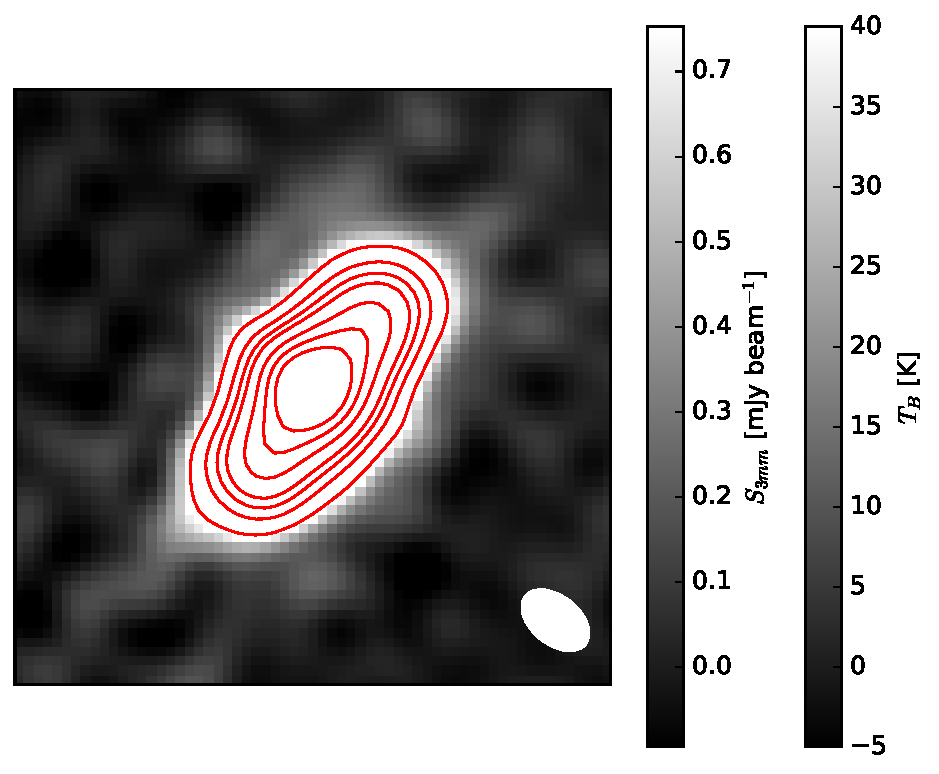
\includegraphics[scale=1,width=3.5in]{figures/OrionSourceI_data_stretched_B3.pdf} }
\subfigure[]{ 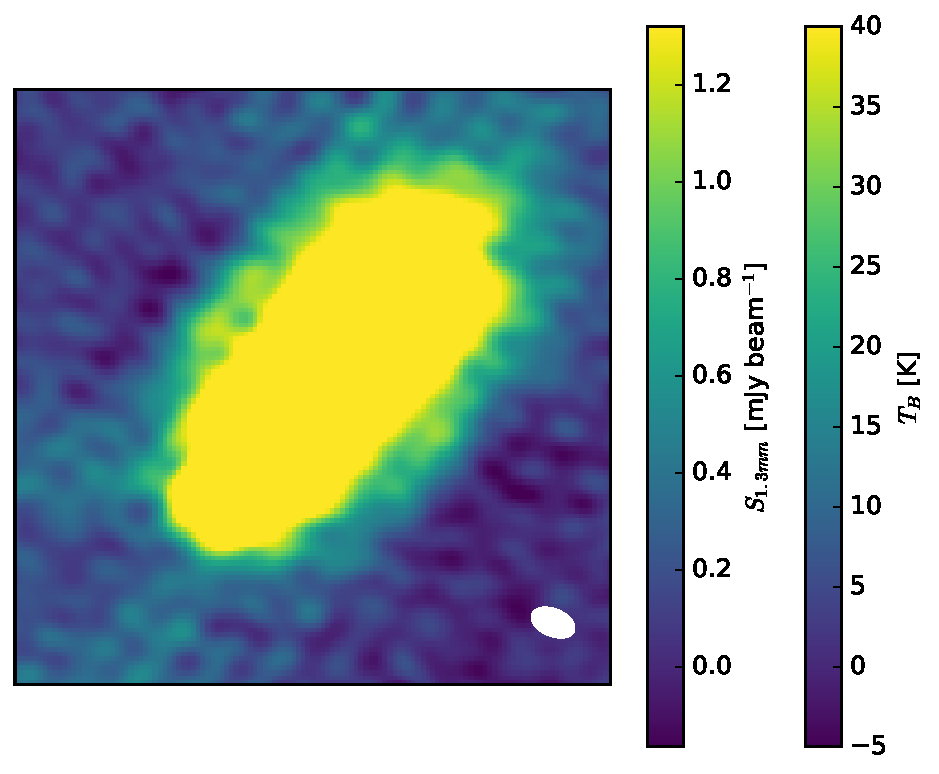
\includegraphics[scale=1,width=3.5in]{figures/OrionSourceI_data_stretched_B6.pdf} }
\caption{The robust -2 continuum image of Orion \sourcei at 3.2 mm (left) and 1.3 mm (right).
The beam is shown
in the bottom right, with size $\Bthreemaj\arcsec\times \Bthreemin\arcsec$ at
PA$=\Bthreepa\degrees$ (3.2 mm, left) and $\Bsixmaj\arcsec\times \Bsixmin\arcsec$ at
PA$=\Bsixpa\degrees$ (1.3 mm, right).
Contours are overlaid at $T_B=$50, 100, 150, 200, 300, 400, and 500 K.
The displayed coordinates are offsets from ICRS 05:35:14.5172 -05:22:30.612
(3.2 mm) and ICRS 05:35:14.5173 -05:22:30.6135 (1.3 mm).
}
\label{fig:continuum_data_B6}
\end{figure*}


% \FigureTwo
% {figures/OrionSourceI_data_B3.pdf}
% {figures/OrionSourceI_data_stretched_B3.pdf}
% {The robust -2 continuum image of Orion \sourcei at 3.3 mm.  The beam is shown
% in the bottom right, with size $\Bthreemaj\arcsec\times \Bthreemin\arcsec$ at
% PA$=\Bthreepa\degrees$.
% }
% {fig:continuum_data_B3}{1}{3.5in}


% \FigureThree
% {figures/SourceI_Disk_model.png}
% {figures/SourceI_Disk_model_bigbeam.png}
% {figures/SourceI_Disk_model_bigbeam_withptsrc.png}
% {continuum modeling}
% {fig:contmodels}{1}{3in}


\subsection{SiO Lines}
We detect several SiO lines, including $^{28}$SiO v=0 and v=1 J=5-4,
the isotopologue $^{29}$SiO v=0 and v=1 J=2-1, and the $^{28}$SiO v=0 and v=1 J=2-1
lines.  Some views of these data are shown
in Appendix \ref{sec:siopv}, but because the emphasis of this work
is not on the outflow, we do not discuss the SiO further here.


\subsection{Water Line}
The next brightest line, after the masing SiO lines, is the \water
$5_{5,0}-6_{4,3}$ line at 232.68670 GHz, with $E_U=3461.9$ K.
\citet{Hirota2012a} detected this line in 2\arcsec resolution ALMA Science
Verification data, but believed it to be masing.  We report here that, because
it is similar in morphology and excitation level to the 336 GHz vibrationally
excited water line reported in \citet{Hirota2014a}, and it has a peak
brightness temperature $\sim1500\pm100$ K (in the robust -2 maps; see Figure
\ref{fig:U1peak}), it is most likely a thermal line.

The water line traces an X-shaped feature above and below the disk, resembling
the overall distribution of SiO masers.  The water is not directly aligned with
the continuum disk (Figures \ref{fig:U1peak} and \ref{fig:h2omom0}), but it
does exhibit emission parallel to the disk at small ($<20$ AU) separation.  The
velocity profile of \water is much better fit by a Keplerian profile than the
SiO thermal or maser emission (see Appendix \ref{sec:siopv}), though this may
be because the SiO is brighter in the outflow than in the disk.
The morphology of this line confirms that it traces both the disk and
the inner rotating outflow discussed by \citet{Hirota2017b} \citep[see
also][]{Kim2008a,Matthews2010a}.

%the SiO is absent from intermediate velocities at
%intermediate separation and is detected at higher velocities and lower
%separations than \water.

Because the water emission is thermal, it exhibits less extreme
brightness fluctuations across the image than the SiO masers, allowing us to
fit an upper-envelope velocity curve in Section \ref{sec:kinematics}.

% {\color{red} To make the above more explicit: a 100 Jy maser will have an
% apparent `envelope' larger than any thermal emission simply because of observational
% effects (convolution with the beam), while for the thermal lines, simply going out
% to a few-sigma threshold is still quite likely to be `line core' emission rather
% than purely beam effects.  We should probably still be deconvolving the beam from
% the envelope-fit estimates, and therefore revise the mass slightly downward.}

% While the continuum disk truncates at r=50 AU, the lines show emission
% beyond this radius, with \water exhibiting emission out to $r\sim100$ AU
% {\color{red} This is a coarse estimate, and the water probably only goes out to
% $r>50$ AU above and below the disk}.

\subsection{Other lines}
\label{sec:otherlines}
Several unidentified lines are observed in  emission at the outer edge of the
continuum disk.  They all share a common morphology, though they vary in
strength.
The peak signal from these lines appears around the $T_B\sim150$ K  contour
in the robust -2 weighted 1.3 mm continuum images
%within the $T_B\gtrsim75$ K contour
(Figure \ref{fig:U1peak}).
There is also emission detected directly above and below the disk at all projected
radii, though it is weaker.  Little line emission is detected where the continuum is
brightest, $T_B\gtrsim300$ K.

The best explanation for these lines is that they trace the outer surface of a
mostly optically thick (in the continuum) disk.  In this scenario,
the lines have an excitation temperature similar to the brightness temperature
of the disk, but have optical depths of order 0.1-1.  
Directly toward the disk
continuum emission peak, since
the line excitation temperature is the same as the background continuum temperature,
$T_{ex}=T_{bg}$, no emission (or absorption) is observed.  Just above and below
the disk midplane continuum peak, the dust column density (and therefore
optical depth) drops rapidly, but the molecular optical depth drops more
slowly, so some emission is still
observed ($T_{ex}\sim200-500$ K, but $\tau_{line}\sim0.1-0.5$, resulting in 
the $T_{B,max} \sim 100$ K observed).  At the disk edges, the column density of
molecular material is higher because we are looking along the tangent of the
disk, so the line optical depth and therefore brightness are greater.

Since these lines only appear immediately around the disk, and in particular
because they peak just outside of the dust emission along the disk axis, they
are the most direct tracers of the disk's kinematics.

% {\color{blue} This paragraph follows from discussion with John.  It might
% be too much detail for a Letter.}
% The lines' kinematic structure suggests they are emitting only from $30~\mathrm{AU}< r <
% 70$ AU.  There are several plausible explanations for the lack of gas
% emission at $r<30-40$ AU: (1) there is no gas at these radii except in the
% optically-thick dust disk, i.e., the gas and dust are well-mixed and the dust
% hides the gas emission (2) the gas is
% heated enough to drop the optical depth in the observed lines by increasing the
% number of available levels in the partition function, decreasing the intensity
% of any given line (3) the molecular line abundance is
% lower closer to the center (e.g., the molecule we observe is dissociated).
% The first explanation is perhaps the simplest, but all three are 
% plausible.


% Their lack of association with the inner disk suggests that they trace the outer
% surface of a mostly optically thick disk.




% If a molecule is at a similar temperature to the dust, but its line approaches
% an optical depth near unity at a lower column density of \hh than the dust,
% it should appear in emission.  These lines therefore appear to trace the disk
% directly and provide the best direct tools for measuring the disk kinematics.



\begin{figure*}[!htp]
\subfigure[]{ 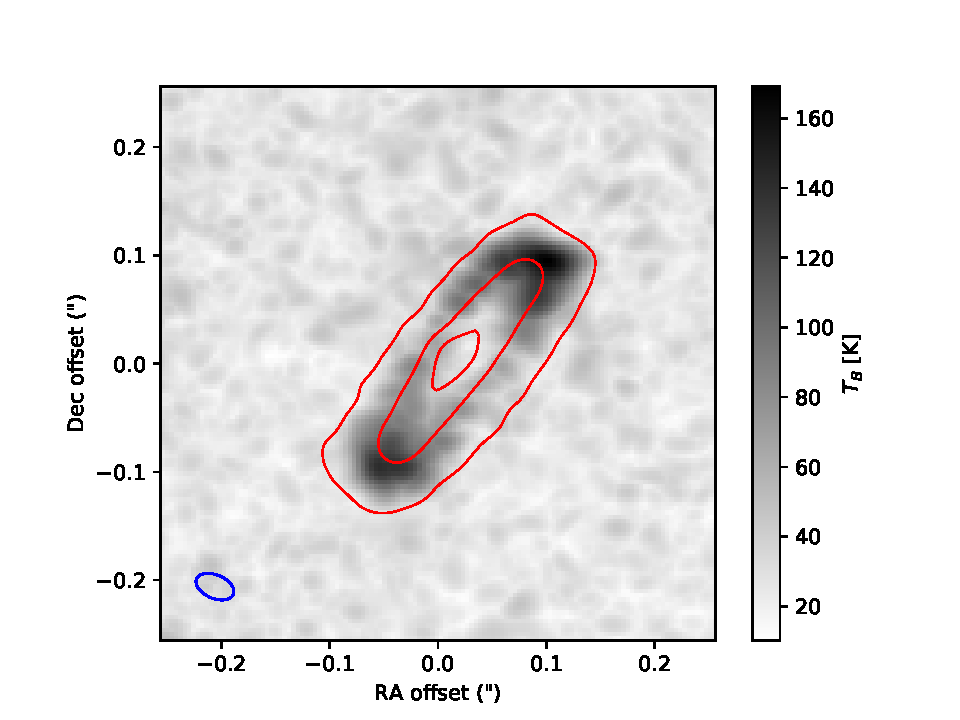
\includegraphics[scale=1,width=2.2in]{{figures/OrionSourceI_Unknown_1_robust0.5.maskedclarkclean10000_medsub_K_peak_offset}.pdf} }
\subfigure[]{ 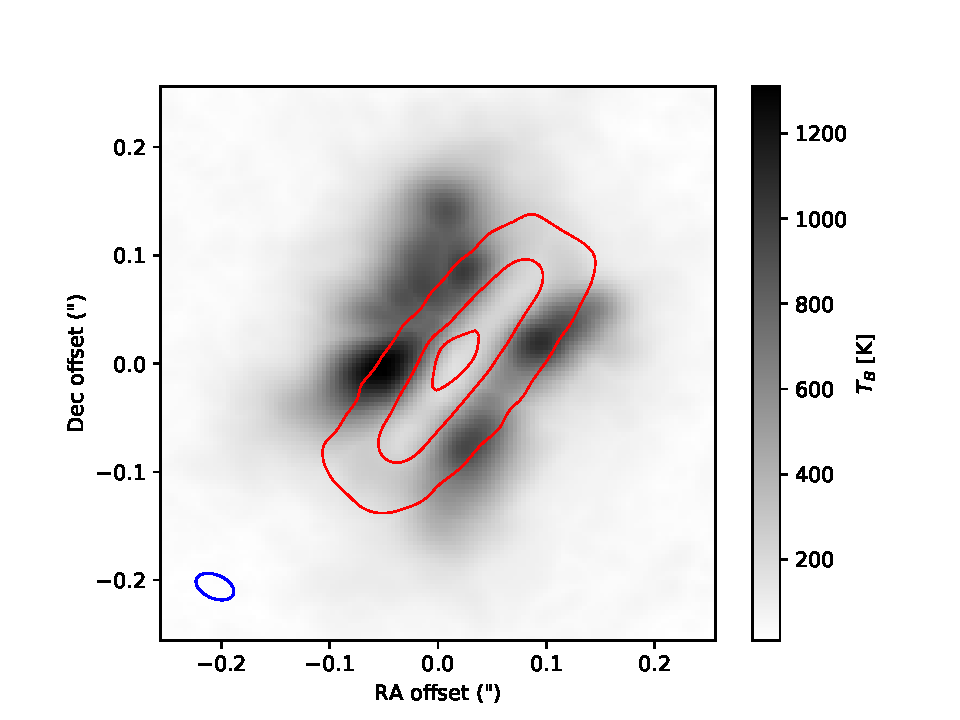
\includegraphics[scale=1,width=2.2in]{{figures/OrionSourceI_H2Ov2=1_5(5,0)-6(4,3)_robust0.5.maskedclarkclean10000_medsub_K_peak_offset}.pdf} }
\subfigure[]{ 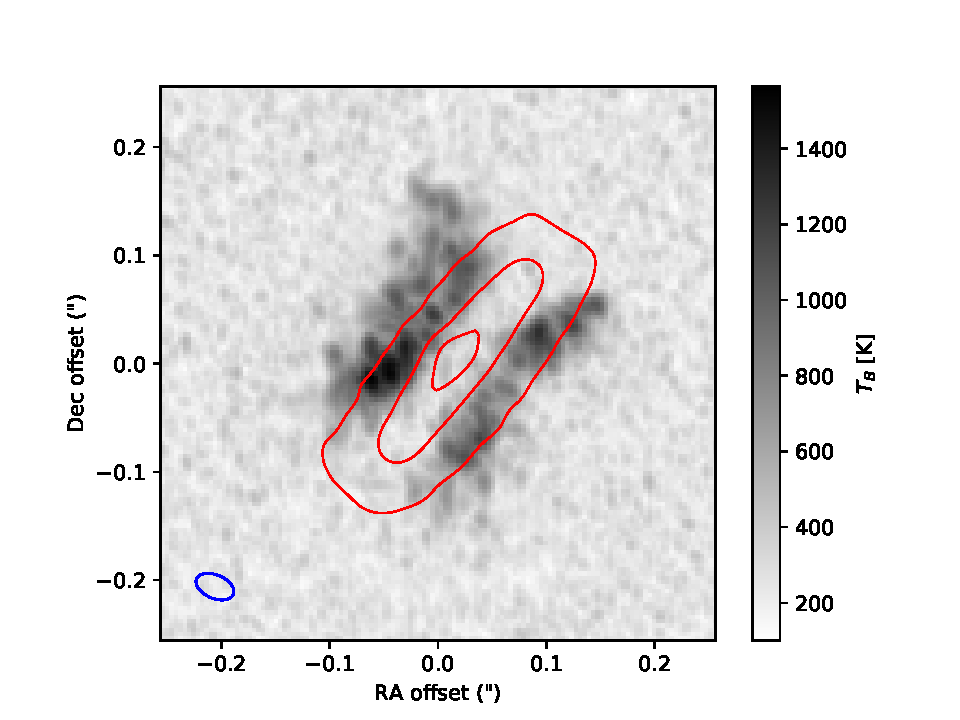
\includegraphics[scale=1,width=2.2in]{{figures/OrionSourceI_H2Ov2=1_5(5,0)-6(4,3)_robust-2.maskedclarkclean10000_medsub_K_peak_offset}.pdf} }
\caption{Peak intensity map of an unknown line (U230.322; left) and the \water
line (middle, right) with continuum overlaid
in red contours at levels of 
50, 150, 300, and 500 K. The \water and unknown line clearly trace different physical structures, as
they exhibit no coincident emission peaks.  The water line does
not exhibit emission directly along the disk midplane.
The left two figures are robust 0.5 weighted images, while the right
is a robust -2 weighted image with higher resolution and poorer
sensitivity.  The U230.322 line is not detected in the robust -2 cubes.
The positions shown are offsets from coordinate ICRS 05:35:14.5184 -05:22:30.6194.
}
\label{fig:U1peak}
\end{figure*}



\subsection{Kinematics: a Keplerian disk}
\label{sec:kinematics}
Following \citet{Seifried2016a}, we measure the outer edge of the detected
emission in a position-velocity (PV) diagram to define the rotation curve
surrounding \sourcei. 
% In this technique,
%The outer envelope of the rotation curve is identified in a position-velocity (PV)
%Diagram extracted along the disk direction.
The emission along each line-of-sight
in the PV diagram is followed from
its peak down to some emission threshold.
We use a threshold of 5-$\sigma$, as was done in \citet{Seifried2016a}, but we assess
the importance of this threshold in Section \ref{sec:errorestimate}.
Additionally, to facilitate direct comparison with
previous works, we use the centroid-of-velocity-channel approach
in Appendix \ref{appendix:centroids} (although 
\citet{Seifried2016a} warn it may underestimate the central mass)
and obtain similar results, albeit from different spectral lines.

Of the detected lines, the \water line spans the widest range of
velocities as a function of radius.  As shown in Figure \ref{fig:h2okepler},
there is \water emission spanning at least radii $r\approx 10$ to 100 AU.  Many
other molecules, most of
which we have not been able to identify, span a range of radii 30-80 AU, while SiS
spans 30 AU to an unconstrained outer radius.   The SiO lines span varying radii,
but they are predominantly detected far from the disk midplane (however,
see Appendix \ref{sec:siopv}, in which SiO also exhibits Keplerian velocity
curves).

We find that a 15 \msun edge-on Keplerian rotation curve fits\footnote{We do
not report best-fit parameters and statistical errors here because the errors
on the outer envelope are poorly characterized and likely dominated by
systematic errors such as channel discretization.  } the outer edge of
the \water line reasonably well (Figure \ref{fig:h2okepler}) and is also an
acceptable match to the outer profiles of the unidentified lines
described in Section \ref{sec:otherlines} and shown in supplemental figures in
Appendix \ref{sec:ulinefigures}.  A lower-mass central source is consistent
with the \water data only if we allow for substantial line broadening driven
by turbulence \citep[but
see][who observe stringent upper limits on turbulence in lower-mass
disks]{Flaherty2017a}. 
% {\color{red}
% Sanity check me here - we want the thermal broadening of \water, $(k_B T / (18
% \mathrm{amu}))^{1/2}$, right?}


A substantially smaller mass, such as the 5-10 \msun suggested previously
\citep{Plambeck2016a,Hirota2014a}, is inconsistent with the data: for models
with such masses, emission is clearly detected outside of the predicted
Keplerian curve.  


\begin{figure*}[!htp]
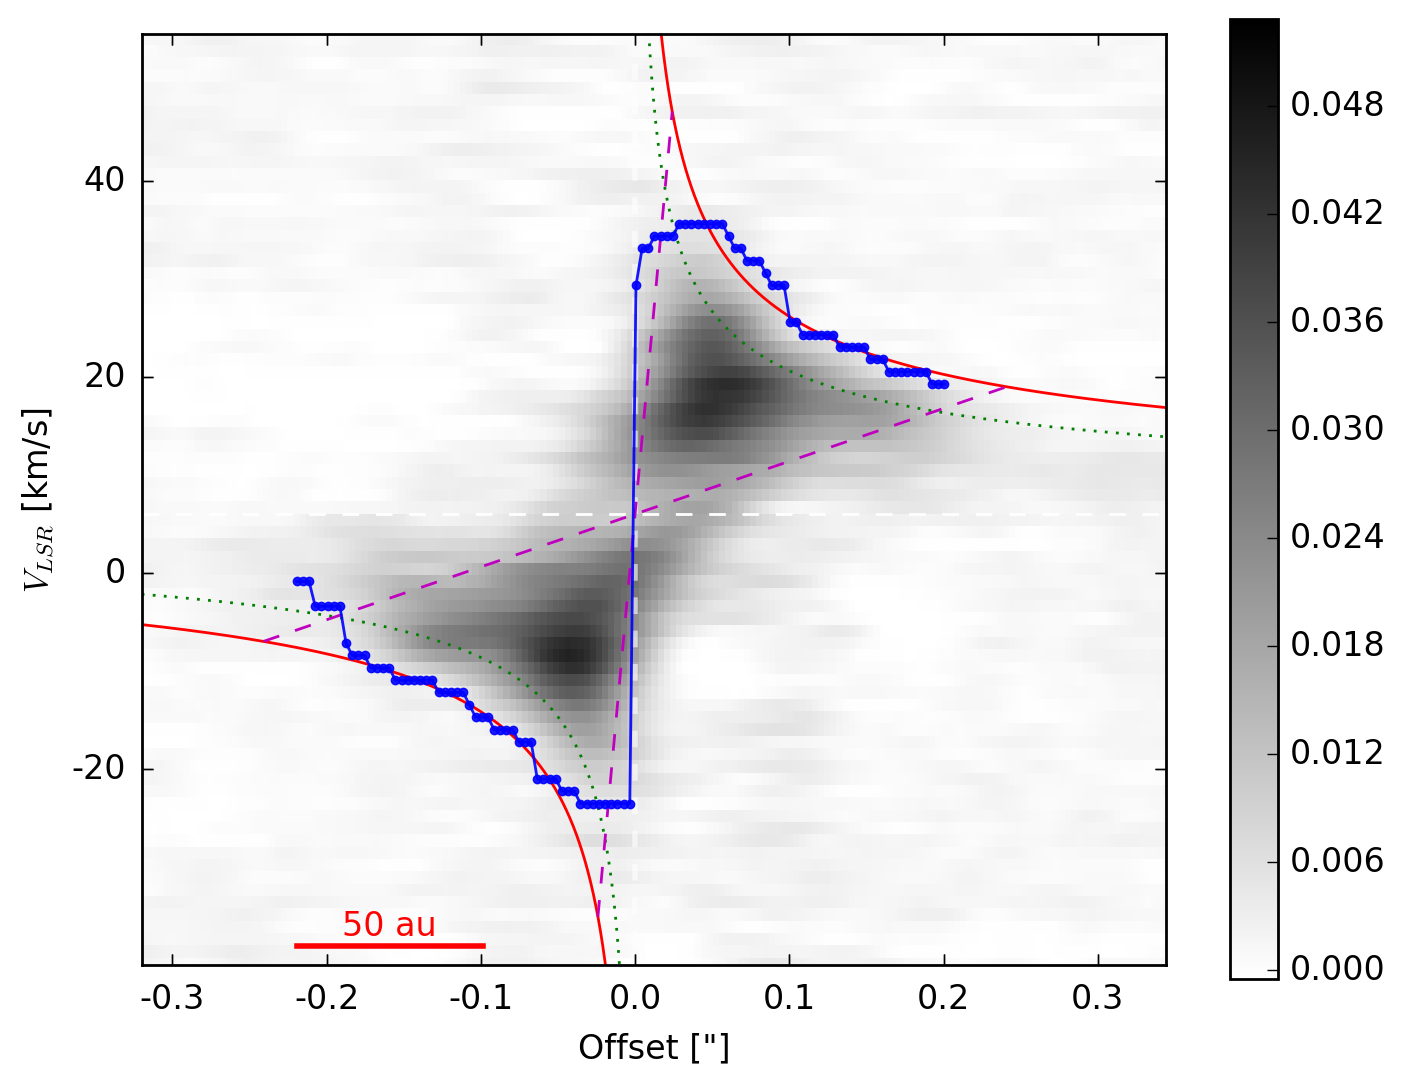
\includegraphics[scale=1,width=7in]{figures/H2O_kepler_SeifriedPlot_0.01arcsec.pdf}
\caption{Position-velocity diagram of \water $5_{5,0}-6_{4,3}$.
The colorbars show average intensity along the extracted region in units
of mJy \perbeam.
The blue line with dots is the outer envelope of the velocity curve
determined using the method of \citet{Seifried2016a}.
The red solid and green dotted curves show the Keplerian velocity profile
surrounding a 15 and 10 \msun central source, respectively.
White dashed lines indicate the adopted source central position
05h35m14.5172s -05d22m30.618s (ICRS)
and central velocity (5.5 \kms).
The purple dashed lines show the full orbital path for radii of
10 and 100 AU and indicate the approximate limits of the disk.
This PV diagram is extracted from the midplane of the robust 0.5 image,
but the emission displayed is beam-smeared from just above and below the
continuum disk.
}
\label{fig:h2okepler}
\end{figure*}


% Our measurements differ from previous works because of our greater resolution
% and sensitivity.  The great sensitivity allows us to detect kinematics in
% thermal lines, while the improved resolution allows us to use the
% max-velocity-envelope method to measure the velocity curve of those lines.  The
% max-velocity-envelope method cannot be applied to maser data, since masers,
% unlike thermal lines, do not trace the full gas velocity profile.


% The main reason our measurements differ from those of \citet{Plambeck2016a},
% \citet{Hirota2014a}, and \citet{Matthews2010a} is that our spatial resolution
% is substantially better.  This improved resolution allows us to use a better
% method to infer the mass from the rotation curve.  Our method is motivated by
% the simulations of \citet{Seifried2016a}, who show that the centroid-based
% method used in previous works (which they were forced to use because of their
% lower spatial resolution) systematically underestimates the central source
% mass.  A detailed comparison of our measurements to those of
% \citet{Plambeck2016a} is given in Appendix \ref{appendix:centroids}, in which
% we conclude that, even using the deprecated method, we infer a mass $M_I \sim
% 15$ \msun.
% 
% {\color{red} Note to coauthors:
% What uncertainties are there in these measurements?
% Do we need to account for turbulent line broadening?
% \citet{Flaherty2017a} suggest that there is negligible turbulence in low-mass disks,
% but what about \sourcei?
% 
% If there's no turbulence, and we assume $T\sim1000$ K, the
% linewidth of \hh is 2.7 \kms, which is enough to lead us to overestimate the mass by a
% non-negligible amount.  Do we need to correct for this by subtracting off (2.7 / 2) \kms
% from the line extrema?  Or, do we assume that the molecules we are detecting have
% much narrower thermal broadening because they come from massive molecules, e.g., \methanol,
% such that the linewidths are $<1 \kms$?
% }

\subsubsection{Examination of alternative velocity profile models}
To support the argument that the velocity profiles are Keplerian, as opposed to
some other power-law profile as has been found for the outer envelopes of
several low-mass YSOs
\citep{Lee2017h,Aso2017b,Ohashi2014a,Lindberg2014a,Murillo2013a}, we show
power-law fits to the outer envelope velocity profile of the \water line
in Figure \ref{fig:h2opowerlaws}.
This figure convincingly demonstrates that
a power law $\alpha=1$ \citep[e.g., as observed in the outer parts of low-mass
YSO disks;][]{Aso2017b} is inconsistent with the data.  While the best-fit
profile of $\alpha\approx0.4$ is slightly shallower than the Keplerian
$\alpha=0.5$ curve, both shallow profiles are consistent with the data.
The limited spectral resolution of our data is evident in this plot, where
there is little separation in velocity from $\sim30-50$ AU; higher
spectral resolution observations or more sophisticated modeling may be able to
provide a tighter constraint on the power-law slope.

% We limit our
% fits to the outer envelope velocity profile, as opposed to the centroid
% velocity profile, both because of the recommendations of \citet{Seifried2016a}
% that the centroid velocities are biased and poorly fit by Keplerian curves, and
% because the centroid velocities of both SiO and \water are not dominated by the
% disk's velocity.  The outer envelope profile, however, appears to be dominated
% by the disk.


\begin{figure}[!htp]
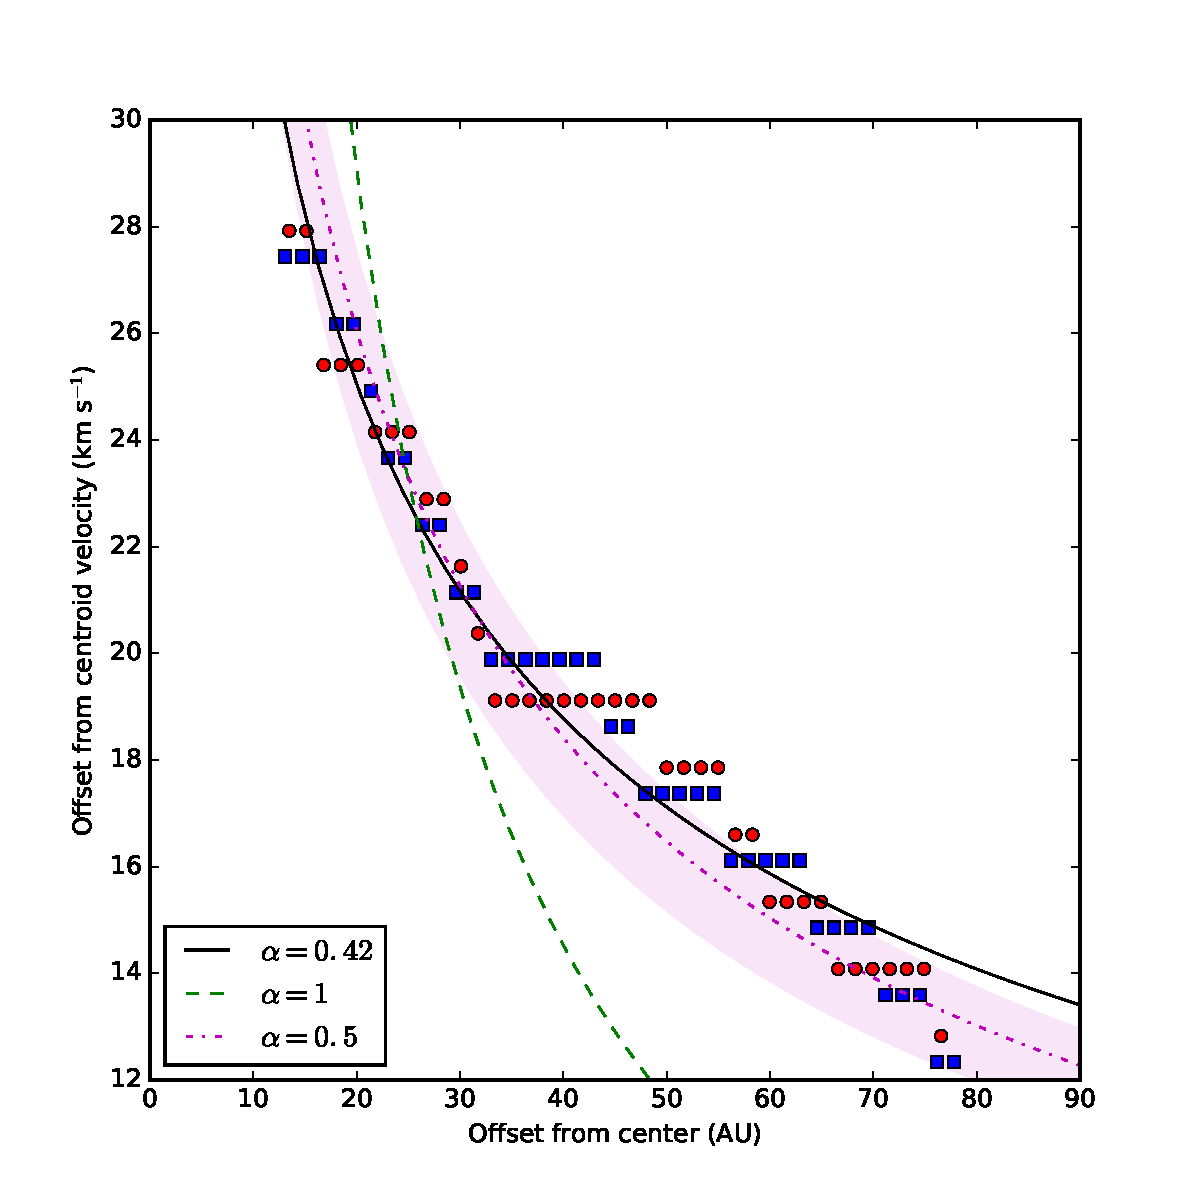
\includegraphics[scale=1,width=3.0in]{figures/bestfit_powerlaw_H2O_kepler_SeifriedPlot_0.01arcsec.pdf}
\caption{Radial profile of the outer-envelope velocity profile extracted from
Figure \ref{fig:h2okepler}b.  The red and blue points represent the redshifted
and blueshifted components of the velocity profile, respectively.  The velocities
are shown relative to the best-fit centroid velocity for the \water line,
$v_{LSR}=5.2$ \kms.  The curves show the best-fit power-law (black solid line)
and the best-fit curves with fixed powerlaw indices of 0.5 (magenta dotted line)
and 1 (green dashed line).  The magenta filled curve shows a powerlaw index
$\alpha=0.5$, i.e., a Keplerian rotation curve, for the range $13 \msun < M <
17 \msun$. }
\label{fig:h2opowerlaws}
\end{figure}


%Figure \ref{fig:h2opowerlaws} shows several power-law profiles superposed on
%the outer-envelope velocity profile.


The mass for the $\alpha=0.5$ curve is $M=15$ \msun; we do not determine
masses for the other models since they are not consistent with a pointlike
gravitational potential.  We show the curves for a central 13-17 \msun source
in filled magenta; since there are many points above the curve, a more massive
central source is plausible, while a less massive source is unlikely.

\subsubsection{An estimate of the error on the mass measurement}
\label{sec:errorestimate}
We  assess the uncertainty introduced by the threshold level adopted in the
velocity envelope profile measurement.  Figure \ref{fig:seifreidthresholderror}
shows the effects of increasing or decreasing the threshold, which is to
decrease or increase the measured mass, respectively.  These figures suggest
that our measurement uncertainty with the PV envelope fitting technique  is
approximately 2 \msun.


\begin{figure*}[!htp]
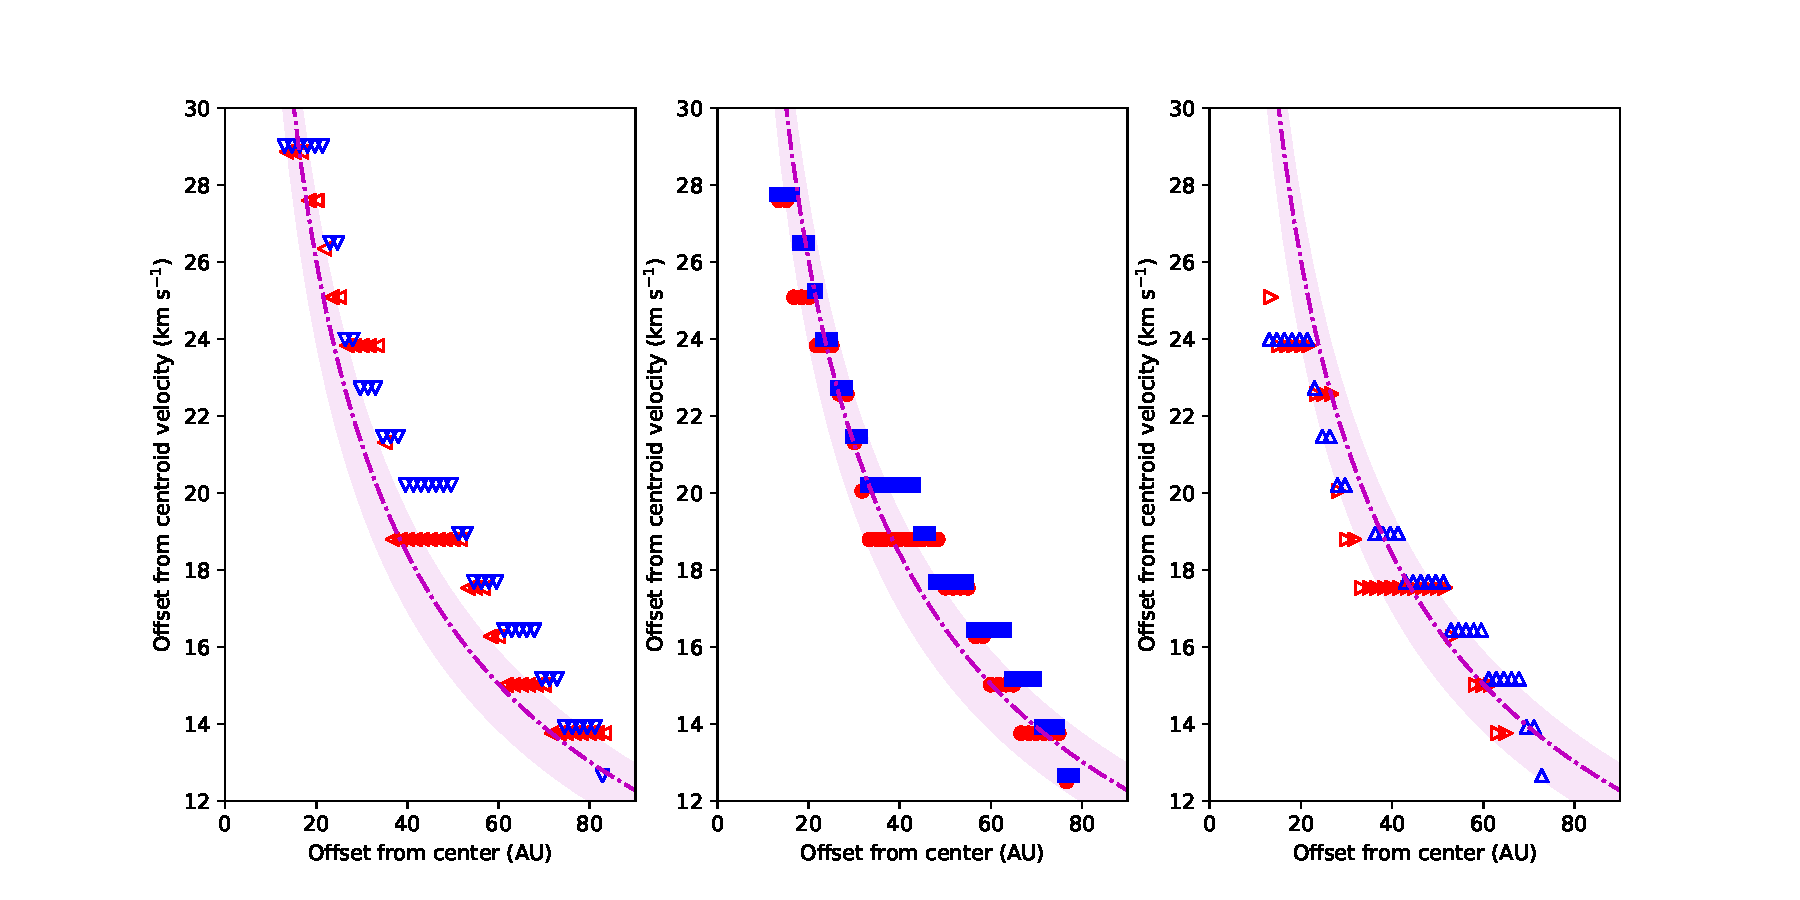
\includegraphics[scale=1,width=7.5in]{figures/outerenvelope_velocity_thresholds_H2O_kepler_SeifriedPlot_0.01arcsec.pdf}
\caption{Demonstration of the effect of a changing threshold in the Seifried method.
The panels show a lower 3-$\sigma$ threshold (left), the adopted 5-$\sigma$
threshold (center), and a higher 7-$\sigma$ threshold (right).  
The magenta highlighted region is the same 13-17 \msun Keplerian curve shown
in Figure \ref{fig:h2opowerlaws}.  
}
\label{fig:seifreidthresholderror}
\end{figure*}



\section{Discussion}
\label{sec:discussion}
\subsection{The mass of \sourcei}
We measure a mass for the object at the center of the disk of $M_I=15$
\msun, which is higher than most measurements previously reported.  Our mass
measurement is higher than previous works in part because our spatial
resolution is high enough to allow a direct fit of the rotation curve to the
outer envelope of an emission line in position-velocity space.
Additionally, though, the greater sensitivity of these observations allowed
us to detect the outer envelope of the \water position-velocity diagram
and detect - and resolve - several unknown lines that directly trace the disk.
The consistency of these new estimates with higher masses than derived from
previous SiO measurements hints that, in this system, SiO chemically selects a
kinemetically distinct region from the disk.

Even if \sourcei consists of an equal-mass binary, this mass measurement
confirms that the Orion Molecular Cloud is presently a region with ongoing
high-mass star formation.
%If the star or stars in \sourcei were below $M<8$
%\msun, Orion might instead have been regarded as a region of past high-mass
%star formation.
% ref to Goddi2011b?

\subsection{The luminosity of \sourcei}
Since we observe an optically thick surface, we can infer the luminosity
required to keep such a surface at the observed $T_{B,1.3 mm}\approx$500 K assuming
it is heated only by radiation.  Taking the disk radius to be 50 AU,
the required central source luminosity is 6500 \lsun.  This estimate
should be taken as a lower limit, since the inner disk is likely to be
optically thick and capable of shielding the outer disk, thereby
keeping the observed $\tau=1$ surface at 1.3 mm cooler than would
be produced by radiative equilibrium with the central star.

\subsection{Properties of the disk}
Our observations yield disk properties nearly identical to those in
\citet{Plambeck2016a}, so we do not revisit their disk mass or density
estimates.  We note, however, that these new observations have sufficient
angular resolution to distinguish the molecular lines that trace the outflow
from those that directly trace the disk.

\subsection{The dynamical decay scenario}
Several authors \citep[][]{Gomez2008a,Goddi2011b,Bally2011a} suggested that
the high proper
motion of \sourcei, BN, and \sourcen, combined with the observed \hh outflow,
implied the outflow and the runaway stars were produced in the same single
event $\sim500$ years ago.  That event was the dynamical decay of a
non-hierarchical multiple system, i.e., it was the interaction of multiple
stars at the center of a small cluster.  More recent observations by
\citet{Luhman2017a} have shown that \sourcen is unlikely to have participated
in this interaction, but instead that \sourcex, another star within the same
field, has high proper motion that points back to the interaction center (Bally et al,
in prep).

\citet{Farias2017b} report that, while any dynamical decay scenario involving
Sources I, X, and BN that can reproduce the observed proper motions are
unlikely, those with a higher mass for \sourcei ($M_I>14$ \msun) are the only
ones capable of producing the observed proper motions\footnote{Their results
are similar to those obtained in \citet{Goddi2011b} and \citet{Moeckel2012b},
but now with \sourcex instead of \sourcen as the third member of the
interaction.}.  Our observed higher mass for \sourcei, $M_I\gtrsim15$ \msun,
therefore implies that the
dynamical interaction scenario remains viable.

% \subsection{The `flyby' scenario}
% \citet{Tan2004a} and \citet{Chatterjee2012a} described a scenario in which BN
% was ejected from the $\theta$1C system and flew through the Orion Hot Core that
% contains \sourcei.   Our observations provide one important constraint on this model:
% the disk position angle.
% The \sourcei disk position angle is  closely aligned to the proper
% motion vector of BN and the vector connecting \sourcei and BN,
% implying that BN played a significant role in the disk's formation.
% This role in turn implies that BN must have come very close to \sourcei,
% within $<100$ AU, and greatly reduces the interaction cross-section
% from a $\theta$1C ejection.


\subsection{Is the disk consistent with the dynamical ejection model?}
\citet{Plambeck2016a} argue that both the mass of \sourcei and the presence of
the disk rule out the dynamical ejection model of \citet{Bally2011a}.  We have
shown that the star is significantly more massive, but what about the disk?

Following \citet{Bally2011a}, we note that the disk truncates at $R<50$
AU.  At this radius, the orbital timescale is $\sim70$ years, so gas at the
disk's outer radius would have had five to ten dynamical times to relax into a
circular disk configuration after the explosive event.

The alignment of \sourcei's disk with the I-BN vector is consistent with a
dynamical interaction between these sources.  If the ejection resulted in
\sourcei and BN being launched in nearly opposite directions from their center
of mass (which must have been moving in the rest frame of the Orion nebula; 
Bally et al. in prep), any material around \sourcei that remained bound would
be dragged in the direction of \sourcei, and would therefore have a resulting
angular momentum vector orthogonal to the direction of motion.  Any material
with
velocity relative to \sourcei 
$$v < v_{esc} = 23 \kms (M_I/15\msun)^{1/2}  (r/50~\mathrm{AU})^{-1/2}$$
would remain bound.
Assuming \sourcei's present-day proper motion of 11.5 \kms reflects its velocity
at the time of ejection, less than half of the original disk mass would
have been lost, while the rest would remain bound (material moving in the
direction directly opposite \sourcei's ejection direction would have net
velocity relative to \sourcei high enough to escape; the greatest mass
loss would occur if the disk was already in the direction of \sourcei's eventual
launch).
% 11.5 km / s = 23 * (200/50)**-0.5
Material outside $R\gtrsim200$ AU would likely all have become unbound, while other
material would be retained in a disk parallel to Source I's proper motion.
%would remain bound, and with \sourcei's present motion of 17 \kms on the sky,
%that implies all mass within the currently observed disk radius would have
%remained with it.


\subsection{The compact source in the disk}
\label{sec:ptsrc}
We have detected a compact (but marginally resolved) source near the center of
the disk at both 3.2 mm and 1.3 mm.  The source has a spectral energy distribution
that is shallow from 3.2 mm to 1.3 mm ($\alpha\approx1.1$).  Since the source is nearly
coincident with an edge-on disk that we show is optically thick at 1.3 mm, it is
likely that the source is thermal but is significantly attenuated by the disk
at 1.3 mm and seen with less attenuation at 3.2 mm.

\citet{Reid2007a} used comparable-resolution 7 mm VLA data to infer
the presence of a 2.2 mJy source at the center of the \sourcei disk.
The compact-source-to-disk flux ratio at 7 mm was $\sim30\%$, substantially
higher than we observe at 1.3 mm and somewhat
higher than at 3.2 mm (Table \ref{tab:continuum_fit_parameters}).  
% -log(2.2/10) / log(7/3)
% -log(2.2/7.3) / log(7/3)
% -log(2.2/7.3) / log(93.3/43.165)
The spectral index of this compact source from 7 to 3.2 mm is $\alpha=1.6$,
approaching that of an optically
thick blackbody.
%{\color{red} NOTE TO COAUTHORS: These numbers have not stayed
%quite as steady as I like; improved fitting dropped the 3.2 mm point-to-total
%from $\sim20\%$ to $\sim13\%$.}
%blackbody, suggesting that the disk is nearly optically thin at 3.2 mm,
%at least along the line of sight toward this object.

The central source has a surface temperature $T\geq1250$ K, the brightness
temperature of a 2.2 mJy source within a $41\times28$ milliarcsecond beam at 7
mm.  If the source is a 5000 K spherical blackbody \citep[e.g.,][]{Testi2010a},
it must have a radius $R=7.5$ AU.  Such a gigantic star is implausible, as it
would produce a luminosity of 1.5\ee{6} \lsun, several orders of magnitude
higher than the total luminosity in the region.  We therefore argue
that this emission source is not a star.

What is the emission mechanism from this central source?
It could simply be hot, optically thick dust that is partly obscured by the
cooler disk at higher frequencies.  The  extension of this `source' along the
disk direction (Appendix \ref{appendix:contmodel}, Figure
\ref{fig:contmodel_residuals_B6}) suggests that we are
seeing the hot inner disk.  As pointed out by \citet{Plambeck2016a}, it is
quite unlikely to be classical free-free emission from protons
and electrons, since there are no detected
recombination lines.  However, it is still plausible that the emission is
produced by brehmsstrahlung emission from HI and \hh
\citep{Reid2007a,Baez-Rubio2018a}.
% {\color{red} This may be an area worth exploring further given
% the existence of \citet{Baez-Rubio2018a}.}

% 3-5 AU is the expected separation of a binary
The source is slightly offset from the center of the disk by $5.8\pm1.5$ AU in
projection\footnote{We measure the errors on the source position by fitting a
2D Gaussian model to an image with the disk model subtracted.  While this approach
yields a useful statistical error, it does not account for the systematic error
introduced by fitting the disk model. }.  This offset,
combined with the source's extent, implies that it is
not a single central source, but
instead is a hot region of the inner disk.  Such an asymmetry in the disk could
be driven either by instability in the disk or, if the central star is a
binary, by the proximity of the more luminous companion.

If this source is an inner edge of the disk, it may imply the presence of a
binary that has cleared the area within $r<6-10$ AU.  Since a tight binary is
one of the expected outcomes of the dynamical interaction scenario
\citep{Goddi2011b}, this
detection of the inner region in dust emission provides additional
circumstantial evidence for that scenario.

If SrcI's central source is a binary, and the measured offset of $\sim5$ AU
between the disk midpoint and the central emission source is real, we can guess
that the binary's orbit is $\lesssim5$ AU.  For such an orbital radius, the
orbital timescale is only $\sim3$ years.   It will therefore be productive to
re-observe \sourcei over the next several years to see if the hot spot moves on
such a timescale.

\section{Conclusions}
\label{sec:conclusions}
We report observations that resolve \sourcei's disk in both continuum
and line emission.  We measure the mass of \sourcei by fitting the 
rotation curve with a Keplerian disk model, finding the following:

\begin{enumerate}
    \item The central source has mass $M=15\pm2$ \msun, where the the error
        bar represents the range of consistent models rather than a typical
        $1-\sigma$ statistical uncertainty.
    \item The \water $5_{5,0}-6_{4,3}$ line is not masing and kinematically
        traces both the upper envelope of the disk and the lower portion of
        the outflow.
    \item We observe several lines that trace the disk kinematics
        directly, though the molecules producing these lines remain
        unidentified.  These lines are visible only toward the outskirts of the
        disk and are morphologically distinct from both the \water and SiO
        lines that follow the outflow.
    \item A compact source in the approximate center of the disk
        is resolved at 1.3 mm, and it is slightly off-center.  It therefore is
        most likely a hot region of the inner disk.  It may be produced
        by time-varying illumination from an unequal mass binary.
\end{enumerate}

The mass we have measured is higher than in several recent publications because
both the resolution and sensivity of our observations were greater.  These new
data allowed us to identify and measure the spectral features that directly
trace the disk kinematics, while previous data convolved the disk and outflow
kinematics.  This higher measured mass implies that the dynamical decay
scenario for the \sourcei - BN - \sourcex system is viable.

\acknowledgements{
This paper makes use of the following ALMA data: ADS/JAO.ALMA\#2016.1.00165.S
ALMA is a partnership of ESO (representing its member states), NSF (USA) and
NINS (Japan), together with NRC (Canada), MOST and ASIAA (Taiwan), and KASI
(Republic of Korea), in cooperation with the Republic of Chile. The Joint ALMA
Observatory is operated by ESO, AUI/NRAO and NAOJ.  The National Radio
Astronomy Observatory is a facility of the National Science Foundation operated
under cooperative agreement by Associated Universities, Inc.}

\software{
The software used to make this version of the paper is available from github at
\url{https://github.com/keflavich/Orion_ALMA_2016.1.00165.S}
(\url{https://doi.org/10.5281/zenodo.1181877}) with hash \githash
(\gitdate).  The tools used include \texttt{spectral-cube}
(\url{https://doi.org/10.5281/zenodo.591639} and
\url{https://github.com/radio-astro-tools/spectral-cube})
and
\texttt{radio-beam} (\url{https://github.com/radio-astro-tools/radio-beam},
\url{https://doi.org/10.5281/zenodo.1181879}) from the
\texttt{radio-astro-tools} package
( \url{radio-astro-tools.github.io}), \texttt{astropy}
\citep{Astropy-Collaboration2013a}, \texttt{astroquery}
(\url{astroquery.readthedocs.io}, \url{https://doi.org/10.5281/zenodo.591669} )
and \texttt{CASA} \citep{McMullin2007a}.
}


\bibliographystyle{aasjournal}
\bibliography{extracted} 
\appendix
% \section{Other unidentified lines with interesting morphology}
% \label{sec:otherlines}
% In this section, we show two of the other unidentified lines that appear to trace
% the disk.  These figures (\ref{fig:U4} and \ref{fig:U5}) show that the lines
% are nearly absent from the continuum-bright disk, but are detected along the upper and
% lower surfaces and at the extrema along the disk.  The associated position-velocity diagrams


\section{Methodological comparison}
\label{appendix:centroids}
To compare fairly with \citet{Hirota2014a} and \citet{Plambeck2016a}, we  used
the centroid-velocity method to measure the central source mass.  In this
approach, we fit two-dimensional Gaussian profiles to each `blob' in each
velocity channel in the PPV cubes of spectral lines.  Unlike previous works, we
have had to fit multiple Gaussians in several channels, since we resolve the
structure and see `blobs' both above and below the disk.  Figures
\ref{fig:velcen_U4}, \ref{fig:velcen_sio}, and \ref{fig:velcen_h2o} show the
results of this analysis.

% {\color{red} Question to coauthors: How should I implement this modeling?
% My current implementation lives at
% \url{https://github.com/keflavich/Orion_ALMA_2016.1.00165.S/blob/master/analysis/edge_on_ring_velocity_model.py},
% and effectively assumes an infinitely small beam.  A larger effective beam will
% have some effect on the observed velocity profile; I believe it will weight
% toward higher velocities, therefore steepening the slope.  I don't incorporate
% line width at all in this analysis, but I can't convince myself it should have
% any effect under the assumption that the disk is symmetric and we are measuring
% centroids.}


We have modeled the velocity profile assuming an edge-on, uniform, optically
thin disk with a sharp central hole and outer truncation.  Position-velocity
curves derived with this approach are shown in the above figures. Figure
\ref{fig:massradiusdemo} shows the curves for a range of masses and radii.
This model approach is the same used by \citet{Plambeck2016a}.  We fit this
model to the centroid data points.  The fits were performed on the
\emph{average} positional offset at each velocity, since for many velocities
there were two or more Gaussian components fitted in the image.  The mass,
inner and outer radius, and centroid velocity were left as free parameters.
The fit results are shown in the legend of Figures 
\ref{fig:velcen_U4} and \ref{fig:velcen_sio}; in Figure \ref{fig:velcen_h2o},
we show only a fiducial model because the best-fit model did not describe
the data well.

The positions of the fitted components are significantly different for each
species, which helps illustrate why previous estimates of \sourcei's mass were
low.  Fits to both the SiO line in Figure \ref{fig:velcen_sio} and water in
Figure \ref{fig:velcen_h2o} have lower masses than the fit to the U232.511 line
in Figure \ref{fig:velcen_U4} that more closely traces the disk.

% The fitted centroid velocities to the SiO and water lines are slightly higher
% than the typically adopted $V_{I,LSR}=5$ \kms; they are  $\approx7$ and
% $\approx6$ \kms for SiO and \water respectively.  We therefore caution that,
% when identifying lines, it would be advisable to include a $\sim2$ \kms
% systematic error on \sourcei's velocity.


% We compared our data to the models adopted by \citet{Plambeck2016a},
% specifically, the 5 and 10 \msun, $20 < R < 50$ AU models.  Neither of these
% reproduce the position-velocity curves we have measured with our
% higher-resolution data.  

% While the
% lower-mass source agrees better with the tilt of the velocity curve, it fails
% to reproduce the high observed maximum velocities.

In the edge-on disk models, different inner-radius cutoffs have an effect on
the inner velocity profile slope similar to changing the central mass, so it is
likely that the disk parameters, rather than the central source mass, dominate
our uncertainties in this approach.  
Figure \ref{fig:massradiusdemo} demonstrates this effect: the inner slope of
a 5 \msun, $20~\mathrm{AU} < r < 50~\mathrm{AU}$ disk is indistinguishable
from a 20 \msun , $30~\mathrm{AU} < r < 80~\mathrm{AU}$ disk, though the latter
extends to higher velocity and radius.

The most important conclusion from this modeling is that the higher-resolution
data yield a higher mass than the original lower-resolution data, favoring a
central star with $M>10$ \msun for all lines, but $M\approx15$ \msun for the
unidentified lines that appear to most closely trace the disk. 
%However, the centroid-based approach
%still appears consistent with a lower mass ($M\lesssim15\msun$) central star
%than the \citet{Seifried2016a} upper-envelope fitting approach.
%The centroid-based approach may be particularly biased to lower masses
%by the existence of an optically thick disk, which will hide the highest
%velocity regions at the center of the disk.
%This remaining
%ambiguity highlights the difficulty of direct mass inference from assumed
%Keplerian velocity curves and the need for more sophisticated disk radiative
%transfer models.


\begin{figure*}[!htp]
\subfigure[]{ 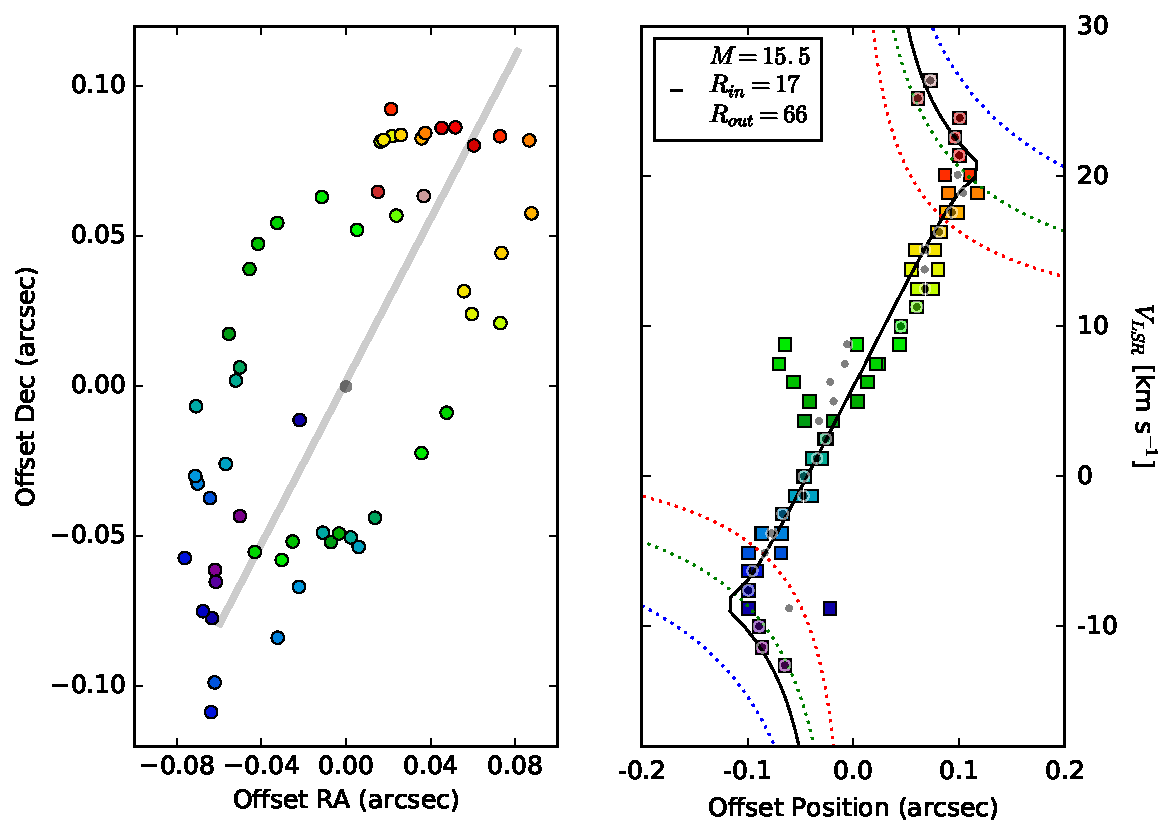
\includegraphics[scale=1,width=3.5in]{figures/Unknown_4_pp_pv_plots_fittedmodel_withavgs.pdf} }
\subfigure[]{ 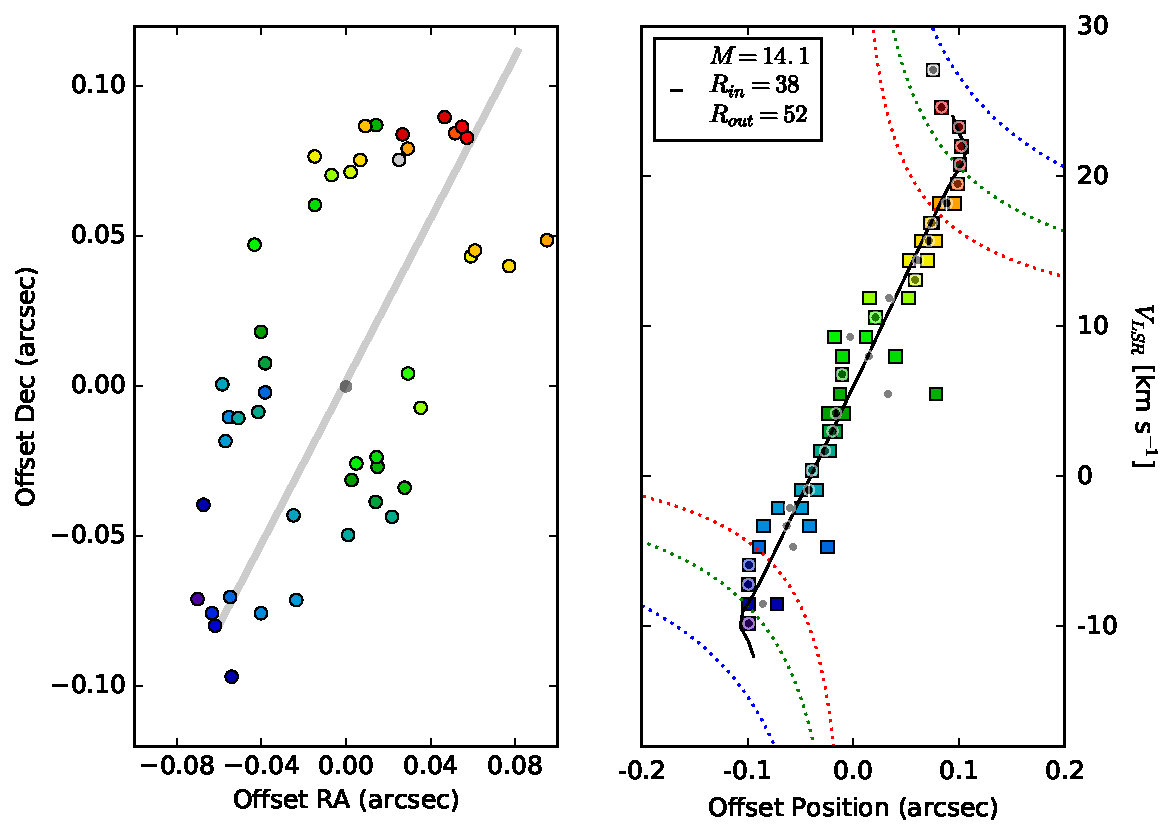
\includegraphics[scale=1,width=3.5in]{figures/Unknown_1_pp_pv_plots_fittedmodel_withavgs.pdf} }
\caption{Results of the centroid-velocity analysis for the U232.511 line (left) and the U230.322 line (right).
The left panel shows the locations of fitted centroids in the position-position
plane relative to the midpoint of the disk.  
The position of the central compact source is
marked with a grey circle at the center.  The grey line indicates the disk
midplane as determined from the continuum modeling.  The circles are colored by
their velocity as indicated in
the right panel.  The right panel shows a position-velocity diagram of these
same centroids.  The dotted external curves show Keplerian velocity profiles
for a  15 \msun (red solid) central source; this curve does \emph{not} represent
what should be observed in a centroid-of-velocity plot.
The black curve shows the predicted centroid velocity profile of an
optically-thin edge-on disk with parameters displayed in the figure.
}
\label{fig:velcen_U4}
\end{figure*}



\begin{figure*}[!htp]
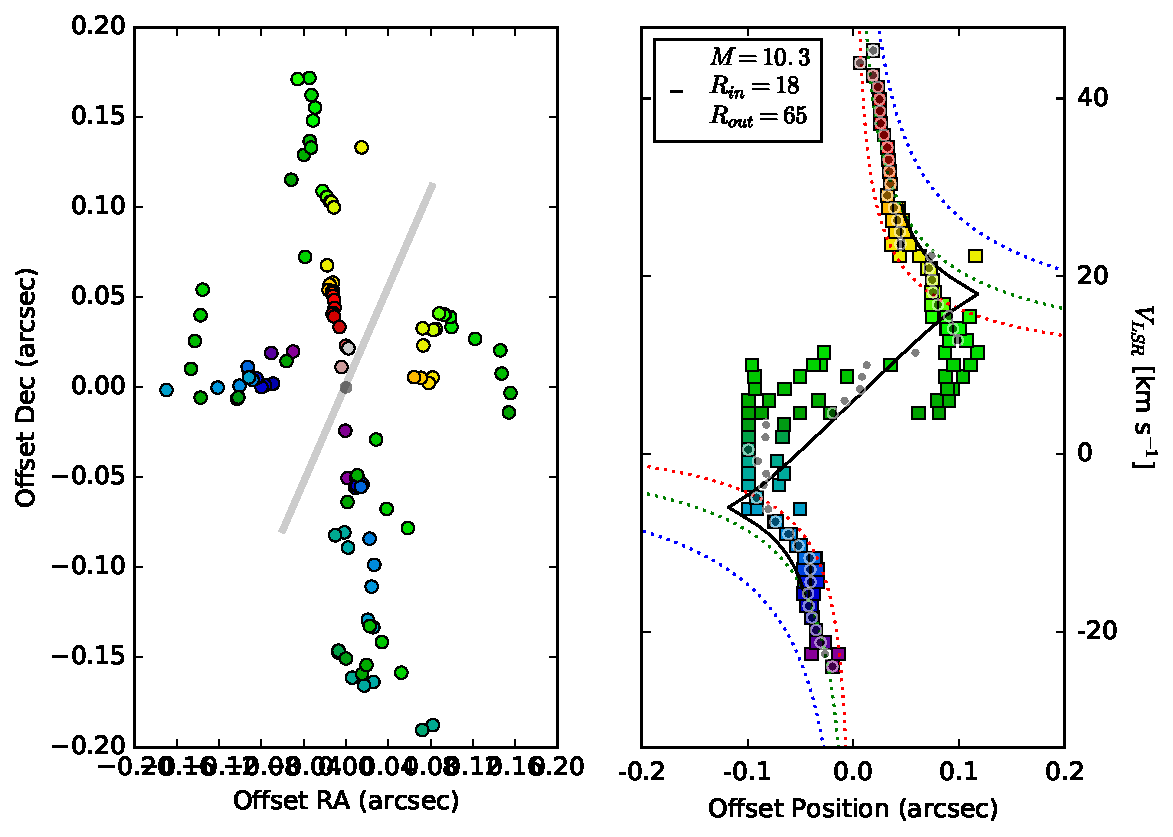
\includegraphics[scale=1,width=6in]{figures/SiOv=1_5-4_pp_pv_plots_fittedmodel_withavgs.pdf}
\caption{Results of the centroid-velocity analysis for the SiO v=1 J=5-4 line.
See Figure \ref{fig:velcen_U4} for details.
Note that the data are inconsistent with the disk model;
the SiO emission fitted here traces the bottom of the outflow
and possibly some components of the disk upper atmosphere.
The average positions at each velocity are closer to a reasonable fit.
}
\label{fig:velcen_sio}
\end{figure*}



\begin{figure*}[!htp]
\includegraphics[scale=1,width=6in]{figures/H2Ov2=1_5(5,0)-6(4,3)_pp_pv_plots.pdf}
\caption{Results of the centroid-velocity analysis for the \water line.
See Figure \ref{fig:velcen_U4} for details.
The model disk fit to these data was a very poor fit, so we
have instead overlaid a model that is \emph{not} a fit to the data
with 15.5 \msun, $r_{inner}=17$ AU, and $r_{outer}=66$ AU in the
right panel.
Note that the centroid positions do not extend as far from
the source center as the unknown lines; this effect is 
a symptom of the blending of lines of sight in the centroid-based approach,
since the \water line's faintest emission can be seen extending to at least as
great a distance from the central source as the unknown lines in the
position-velocity diagrams.
}
\label{fig:velcen_h2o}
\end{figure*}



\begin{figure}[!htp]
\includegraphics[scale=1,width=3.0in]{figures/radius_mass_demo.pdf}
\caption{Plots of the predicted centroid rotation curves for different masses
and inner and outer radial cutoffs.  As discussed in Appendix \ref{appendix:centroids},
this figure illustrates the ambiguity between the radial extent of the disk and
the mass of the central source, since an $M=5$ \msun central source with a
$20<R<50$ AU disk has the same slope in the inner part as a $M=20$ \msun source
with a $30<R<80$ AU disk.
}
\label{fig:massradiusdemo}
\end{figure}


% \section{Inset figure of the 3.2 mm data}

\subsection{A demonstration of issues with the centroid-of-velocity method}
Figure \ref{fig:h2opvfailuremode} shows an example of how the
centroid-of-velocity approach produces lower mass fits for some lines,
particularly \water and SiO.  The figure shows both the optically thin edge-on
disk model and the midplane-extracted position-velocity diagram with overlaid
centroid fits.  The centroid fits notably do not extend nearly as far as
emission is visible.  This discrepancy results from the midplane emission being
much fainter than some of the off-plane emission.


\begin{figure*}[!htp]
\includegraphics[scale=1,width=6in]{figures/H2Ov2=1_5(5,0)-6(4,3)_pp_pv_plots_fittedmodel_15msun_withavgs_comparepv.pdf}
\caption{A figure showing the edge-on disk model used to fit the centroid-of-velocity curves with
$M=15 \msun$, $r_{in}=25$ AU, and $r_{out}=65$ AU (left) and the centroid-of-velocity measurements
overlaid on the midplane position-velocity diagram of the \water line (right).}
\label{fig:h2opvfailuremode}
\end{figure*}


By contrast, a similar side-by-side comparison of the edge-on optically thin
model with the U232.511 line reveals a better match.  In Figure
\ref{fig:u4pvmodelcomparison}, the overall structure of the observed
position-velocity diagram is well-matched to the model.

% The discrepancy in
% intensity, in which the inner part of the disk is fainter in the observations
% than in the naive model, is an optical depth effect.
% The inner disk is optically thick, blocking emission at all velocities in the
% inner portion of the disk in projection.  We therefore see mostly, but not
% entirely, the optically thin (in the continuum) outer edge of the disk.




\begin{figure*}[!htp]
\includegraphics[scale=1,width=6in]{figures/Unknown_4_pp_pv_plots_fittedmodel_15msun_withavgs_comparepv.pdf}
\caption{A figure showing the edge-on disk model used to fit the centroid-of-velocity curves with
$M=15 \msun$, $r_{in}=25$ AU, and $r_{out}=65$ AU (left) and the centroid-of-velocity measurements
overlaid on the midplane position-velocity diagram of the U232.511 line (right).}
\label{fig:u4pvmodelcomparison}
\end{figure*}


\section{A deeper examination of the water line: Evidence that it traces the disk kinematics}
\label{sec:waterlinerevisited}
The \water-derived mass presented in Section \ref{sec:kinematics} relies on the
\water line tracing the disk kinematics.  Since the \water clearly also
traces the outflow, showing the same X-shaped morphology as the SiO, it does
not trace just the disk.

Nonetheless, the midplane position-velocity slice of the \water line does
appear to genuinely trace disk kinematics.  Qualitatively, the PV diagram
appears exactly as expected for a disk with an inner and out radial cutoff.

To assess possible contamination from the outflow, we compare position velocity
slices at different vertical displacements from the disk center in Figure
\ref{fig:waterpvheights}.
The left panel shows the kinematic signature we attribute to the disk, which
closely resembles that predicted for a pure Keplerian rotation curve.
In contrast, the middle panel is likely
dominated by outflow emission, since it shows material 0.05-0.1\arcsec (20-40
AU) above the disk, i.e., just outside the 1-$\sigma$ height of the continuum
disk.  
While the outflow continues to show some motion similar to that of the disk, it
lacks the characteristic convex shape of a Keplerian orbit at higher velocities
and separation.
Finally, the rightmost panel shows that the water emission nearly disappears
at heights $h>0.1\arcsec=40$ AU while the maximum velocities observed get
smaller ($dv < 10$ \kms), suggesting that rotation slows in the outflow.

Figure \ref{fig:waterpvheights} also characterizes some of the `forbidden' velocity
components, i.e., those seen in quadrants 2 and 4.  These components get stronger
at higher vertical positions on the disk, implying that they come from the outflow,
not the disk.
The ``ring'' shape observed in the high-latitude figures indicates the outflow
is expanding \citep[see, e.g., the model in supplementary figure 1
of][]{Hirota2017b}.
The velocity asymmetry, which shows an excess toward the red side of the disk
and outflow, is also present in SiO.  We do not have a straightforward
explanation for this asymmetry except to assert that it implies an
asymmetry in the direction of mass ejection in the outflow.
These velocity components are unlikely to be produced by infall motions, since
they are observed perpendicular to the disk along the direction of the outflow.
%{\color{red} Any ideas why the redshifted side is brighter and
%`more extended' (in pv space) than the blueshifted?}


\begin{figure*}[!htp]
\subfigure[]{ \includegraphics[scale=1,width=2.2in]{figures/keplercurves_sourceI_H2Ov2=1_5(5,0)-6(4,3)_B6_robust-2_diskpv_0.1.pdf} }
\subfigure[]{ \includegraphics[scale=1,width=2.2in]{figures/keplercurves_sourceI_H2Ov2=1_5(5,0)-6(4,3)_robust-2_diskpv_0.2-0.1.pdf} }
\subfigure[]{ \includegraphics[scale=1,width=2.2in]{figures/keplercurves_sourceI_H2Ov2=1_5(5,0)-6(4,3)_robust-2_diskpv_0.3-0.2.pdf} }
\caption{Position-velocity slices of the \water $5_{5,0}-6_{4,3}$ line at different
heights above the disk plane from the robust -2 data cube.  The left panel
shows the inner 0.1\arcsec (i.e., near the midplane, $|h| < 0.05\arcsec$,
$|h|<20$ AU), the middle shows the range $0.05\arcsec < |h| < 0.1$\arcsec, and
the right shows the range $0.1\arcsec < |h| < 0.15\arcsec$.  All three panels
show averages over the specified range, with the colorbar showing intensity in
mJy \perbeam.  The red solid lines show the Keplerian
profile for a 15 \msun
central source, and the purple dashed lines show the orbital
track for a particle at 30 and 80 AU for such a source; these are included
primarily to guide the eye.  The middle and right panel are dominated by the
outflow, while the left panel is dominated by the Keplerian orbital profile.
}
\label{fig:waterpvheights}
\end{figure*}


% \FigureThree
% {figures/keplercurves_sourceI_H2Ov2=1_5(5,0)-6(4,3)_B6_robust0.5_diskpv_0.1.pdf}
% {figures/keplercurves_sourceI_H2Ov2=1_5(5,0)-6(4,3)_robust0.5_diskpv_0.2-0.1.pdf}
% {figures/keplercurves_sourceI_H2Ov2=1_5(5,0)-6(4,3)_robust0.5_diskpv_0.3-0.2.pdf}
% {{\color{blue} Same as Figure \ref{fig:waterpvheights}, but
% for robust 0.5.  This is included only for coauthors to have a look at;
% I'll remove it from the final paper.  It shows that some of the features 
% we're looking at really demand the highest resolution.}  Position-velocity
% slices of the \water
% $5_{5,0}-6_{4,3}$ line at different heights above the disk plane from the
% robust 0.5 data cube.  The left panel shows the inner 0.1\arcsec (i.e., near
% the midplane, $|h| < 0.05\arcsec$, $|h|<20$ AU), the middle shows the range
% $0.05\arcsec < |h| < 0.1$\arcsec, and the right shows the range $0.1\arcsec <
% |h| < 0.15\arcsec$.  All three panels show averages over the specified range,
% with the colorbar showing intensity in
% mJy \perbeam.  The red solid lines show the Keplerian profile for a 15 \msun
% central source and the purple dashed lines show the orbital track for a
% particle at 30 and 80 AU for such a source; these are included primarily
% to guide the eye.  The middle and right panel are dominated by the outflow,
% while the left panel is dominated by the Keplerian orbital profile.
% }
% {fig:waterpvheightsr05}{1}{2.2in}


\begin{figure*}[!htp]
\subfigure[]{ \includegraphics[scale=1,width=3.5in]{figures/H2O_kepler_SeifriedPlot_0.1arcsec_robust-2.pdf} }
\subfigure[]{ \includegraphics[scale=1,width=3.5in]{figures/H2O_kepler_SeifriedPlot_0.2arcsec_robust-2.pdf} }
\caption{
Duplicate of Figure \ref{fig:h2okepler} for robust -2 data.
The left figure shows the range $h=\pm0.05\arcsec$, and the right right shows
$h=\pm0.1\arcsec$.
}
\label{fig:h2okepler_rm2}
\end{figure*}


\section{The SiO outflow in PV space}
\label{sec:siopv}
To illustrate the change in velocity structure with height from the disk, 
we show position-velocity diagrams of SiO v=0 J=5-4 in Figure \ref{fig:siopv}.
These images are extracted from equal distances above and below
the disk midplane.  At greater distances from the midplane, the high-velocity,
low-separation features fade out, while more low-velocity material
becomes visible at larger separations.  In the innermost slice, which shows the
SiO emission that just skirts the edges of the disk, the velocity curve is 
consistent with the 15 \msun Keplerian curve overlaid.


\begin{figure*}[!htp]
\subfigure[]{ \includegraphics[scale=1,width=0.23\textwidth]{figures/keplercurves_sourceI_SiOv=0_5-4_B6_robust-2_diskpv_0.1.pdf} }
\subfigure[]{ \includegraphics[scale=1,width=0.23\textwidth]{figures/keplercurves_sourceI_SiOv=0_5-4_robust-2_diskpv_0.2-0.1.pdf} }
\subfigure[]{ \includegraphics[scale=1,width=0.23\textwidth]{figures/keplercurves_sourceI_SiOv=0_5-4_robust-2_diskpv_0.3-0.2.pdf} }
\subfigure[]{ \includegraphics[scale=1,width=0.23\textwidth]{figures/keplercurves_sourceI_SiOv=0_5-4_robust-2_diskpv_0.4-0.3.pdf} }
\caption{Position-velocity slices of SiO v=0 J=5-4 along the disk direction at four heights:
(a) $|h|<0.05\arcsec$,
(b) $0.05\arcsec<|h|<0.1\arcsec$,
(c) $0.1\arcsec<|h|<0.15\arcsec$,
(d) $0.15\arcsec<|h|<0.2\arcsec$.
These images are produced from the robust -2 weighted cubes.
The missing emission around $v=0$ \kms is likely caused by image filtering
effects; at these velocities, there is extended, smooth SiO emission from the
surrounding cloud.
}
\label{fig:siopv}
\end{figure*}



\begin{figure*}[!htp]
\subfigure[]{ \includegraphics[scale=1,width=0.23\textwidth]{figures/keplercurves_sourceI_29SiOv=0_5-4_B6_robust-2_diskpv_0.1.pdf} }
\subfigure[]{ \includegraphics[scale=1,width=0.23\textwidth]{figures/keplercurves_sourceI_29SiOv=0_5-4_robust-2_diskpv_0.2-0.1.pdf} }
\subfigure[]{ \includegraphics[scale=1,width=0.23\textwidth]{figures/keplercurves_sourceI_29SiOv=0_5-4_robust-2_diskpv_0.3-0.2.pdf} }
\subfigure[]{ \includegraphics[scale=1,width=0.23\textwidth]{figures/keplercurves_sourceI_29SiOv=0_5-4_robust-2_diskpv_0.4-0.3.pdf} }
\caption{Position-velocity slices of $^{29}$SiO v=0 J=5-4 along the disk direction at four heights:
(a) $|h|<0.05\arcsec$,
(b) $0.05\arcsec<|h|<0.1\arcsec$,
(c) $0.1\arcsec<|h|<0.15\arcsec$,
(d) $0.15\arcsec<|h|<0.2\arcsec$.
These images are produced from the robust -2 weighted cubes.
While similar to the $^{28}$SiO shown in Figure \ref{fig:siopv},
there is a remarkable position-velocity ring at high elevations
that is coincident with many of the SiO and \water masers.
}
\label{fig:29siopv}
\end{figure*}


\section{Stacked Spectra}
\label{sec:stackedspectra}
We reported the detection of several unidentified lines.
%We have not identified any of the carrier species of these lines.
To measure their frequencies precisely, we performed a stacking
analysis in which we adopt the velocity field of the U232.511 line,
shift all spectra across the disk to the same velocity frame, and average them.
We stacked the robust 0.5 cubes, as the surface brightness sensitivity
of the robust -2 cubes was too poor to justify stacking.
We then fit the lines with Gaussians to determine their centroid frequency.
We searched within a narrow range of velocities ($v_{LSR}=3-8$ \kms)
for known lines in the Splatalogue collection of line catalogs using
\texttt{astroquery}.
While many of the lines have plausible carriers within 1-2 \kms, such as
highly-excited CH$_3$OCHO or variants of SO$_2$, there is no consistent pattern
to the detected lines and no individual species can explain more than a few of
the observed lines.  These disk-averaged spectra are shown in Figure \ref{fig:stackplots_labeled}
with the lines labeled.

We list the line frequencies (which we use as line names), fitted Gaussian
widths, and fitted amplitudes from the stacked spectra in Table
\ref{tab:unknown_line_frequencies}.

\begin{table*}[htp]
\centering
\caption{Unknown Line Frequencies}
\begin{tabular}{cccc}
\label{tab:unknown_line_frequencies}
Line Name & Frequency & Fitted Width & Fitted Amplitude \\
 & $\mathrm{GHz}$ & $\mathrm{km\,s^{-1}}$ & $\mathrm{mJy}$ \\
\hline
U214.549 & 214.549 & 4.1 & 0.7 \\
U214.637 & 214.637 & 3.2 & 0.3 \\
U214.742 & 214.742 & - & - \\
U214.940 & 214.940 & 4.3 & 4.6 \\
U215.009 & 215.009 & 4.6 & 2.7 \\
U217.229 & 217.229 & 2.6 & 1.3 \\
U217.547 & 217.547 & 6.8 & 1.2 \\
U217.666 & 217.666 & 7.2 & 1.1 \\
U217.980 & 217.980 & 5.2 & 5.6 \\
U218.584 & 218.584 & 4.5 & 1.6 \\
U229.247 & 229.247 & 4.8 & 5.9 \\
U229.550 & 229.550 & 8.0 & 1.1 \\
U229.682 & 229.682 & 15.5 & 3.0 \\
U229.819 & 229.819 & 4.7 & 1.8 \\
U230.322 & 230.322 & 4.7 & 3.8 \\
U230.726 & 230.726 & 5.8 & 1.5 \\
U230.780 & 230.780 & 6.7 & 5.1 \\
U230.966 & 230.966 & 10.4 & 1.1 \\
U232.163 & 232.163 & 4.2 & 1.5 \\
U232.511 & 232.511 & 6.7 & 6.2 \\
U232.634 & 232.634 & 7.8 & 0.8 \\
U233.171 & 233.171 & 4.2 & 2.3 \\
U233.608 & 233.608 & 6.8 & 1.5 \\
\hline
\end{tabular}

\par The frequencies listed have a systematic uncertainty of about 2 \kms (1.5 MHz) because they are referenced to the U232.511 line, which has an unknown rest frequency.  The rest frequency used for the U232.511 line was selected to maximize the symmetry of the emission around 5 \kms.  Some lines were detected in only part of the disk and therefore had bad or malformed profiles in the stacked spectrum; these have fits marked with -'s.
\end{table*}
 
%The stacked spectra are shown, with labels,
%in Appendix \ref{sec:stackedspectra}.
%As described in Section \ref{sec:otherlines}, we performed a line-stacking
%analysis by measuring the velocity field of the U232.511 line, shifting all
%spectra across the disk to a common velocity frame, and averaging them.



\begin{figure*}[!htp]
\subfigure[]{ \includegraphics[scale=0.5,width=0.6\linewidth]{figures/lines_labeled_spw0_B6_yzoom.pdf} }
\vspace{0.001mm} \\
\subfigure[]{ \includegraphics[scale=0.5,width=0.6\linewidth]{figures/lines_labeled_spw1_B6_yzoom.pdf} }
\vspace{0.001mm} \\
\subfigure[]{ \includegraphics[scale=0.5,width=0.6\linewidth]{figures/lines_labeled_spw2_B6_yzoom.pdf} }
\vspace{0.001mm} \\
\subfigure[]{ \includegraphics[scale=0.5,width=0.6\linewidth]{figures/lines_labeled_spw3_B6_yzoom.pdf} }
\vspace{0.001mm}
\caption{Plots of the stacked spectra from spectral windows 0, 1, 2, and 3 (see Table \ref{tab:cube_metadata})
with detected lines labeled.  The spectra are shown with the same y-axis limits; bright SiO and \water
emission is cut off.  In spectral window 2, the region around 215.5-215.6 GHz, near the SiO v=1 J=5-4
maser line (which is the brightest line we detect) is affected by imaging artifacts from the cleaning
process.}
\label{fig:stackplots_labeled}
\end{figure*}


\section{Continuum Modeling Figures}
\label{appendix:contmodel}
In this appendix, we show figures illustrating the continuum modeling process.
Figures \ref{fig:contmodel_residuals_B6} and \ref{fig:contmodel_residuals_B3}
show the model and residuals for the band 6 and band 3 data, highlighting the
significantly improved fit as more model parameters are added.

In Figure \ref{fig:contmodel_residuals_B6}, the apparent point sources at the
edge of the disk in the central column are artificial features introduced by
the model; since the model is forced to be smooth, the best-fit model is one
that is more centrally peaked, which results in an under-prediction of the disk
brightness toward the edges.  

Also in this figure, there appears to be a faint `halo' of emission at the
$\sim30$ K level around the modeled region.  The halo is asymmetric, with a
greater extent toward the southwest.  If this feature is not an artifact of the
data reduction, which we cannot rule out, it is likely to be from optically
thin dust above and below the disk, since it is not detected in the 3.2 mm data.



\begin{figure*}[!htp]
\includegraphics[scale=1,width=7.5in]{figures/models_and_residuals_B6.pdf}
\caption{A series of plots showing the band 6 continuum models used and their residuals.
The top row shows the models, starting from a simple 1D linear model convolved
with the beam (left), continuing with a disk smoothed with a broader beam to
account for scale height (middle), and finally a version of the middle model
with a smeared point source added (right).  The fit parameters are given in Table
\ref{tab:continuum_fit_parameters}.  The second and third row show the
residuals (data - model) for each of the models in the top row; the bottom row
uses a narrow linear scale to emphasize the lower-amplitude residuals, while
the top two use an arcsinh stretch to display the full dynamic range.
}
\label{fig:contmodel_residuals_B6}
\end{figure*}




\begin{figure*}[!htp]
\includegraphics[scale=1,width=7.5in]{figures/models_and_residuals_B3.pdf}
\caption{A series of plots showing the band 3 continuum models used and their residuals.
See the caption of Figure \ref{fig:contmodel_residuals_B6} for details.
}
\label{fig:contmodel_residuals_B3}
\end{figure*}


\section{Additional figures showing the disk}
\label{sec:ulinefigures}
We include several additional figures showing the disk moment 0 maps and
position-velocity profiles for some other unknown lines.  These figures show
that the lines displayed in the main text are not unique.

Figure \ref{fig:h2omom0} shows moment 0 maps, which provide a slightly
different view from the peak intensity maps shown in Figure \ref{fig:U1peak}.
Figures \ref{fig:U4} and \ref{fig:U5} show peak intensity, moment 0, and
position-velocity maps of the U232.511 and U217.980 lines.


\begin{figure*}[!htp]
\subfigure[]{ \includegraphics[scale=1,width=2.2in]{{figures/OrionSourceI_Unknown_1_robust0.5.maskedclarkclean10000_medsub_K_moment0_offset}.pdf} }
\subfigure[]{ \includegraphics[scale=1,width=2.2in]{{figures/OrionSourceI_H2Ov2=1_5(5,0)-6(4,3)_robust0.5.maskedclarkclean10000_medsub_K_moment0_offset}.pdf} }
\subfigure[]{ \includegraphics[scale=1,width=2.2in]{{figures/OrionSourceI_H2Ov2=1_5(5,0)-6(4,3)_robust-2.maskedclarkclean10000_medsub_K_moment0_offset}.pdf} }
\caption{Moment-0 (integrated intensity) map of the U230.322 (left) and \water (middle,
right) line with continuum overlaid in contours.  Continuum contours
from the robust -2 map are shown
in red at levels of 
50, 150, 300, and 500 K.
The left two figures are robust 0.5 weighted images, while the right
is a robust -2 weighted image with higher resolution and poorer
sensitivity.  The U230.322 line is not detected in the robust -2 cubes.
}
\label{fig:h2omom0}
\end{figure*}



\begin{figure*}[!htp]
\subfigure[]{ \includegraphics[scale=1,width=2.25in]{{figures/OrionSourceI_Unknown_4_robust0.5.maskedclarkclean10000_medsub_K_moment0_offset}.pdf} }
\subfigure[]{ \includegraphics[scale=1,width=2.25in]{{figures/OrionSourceI_Unknown_4_robust0.5.maskedclarkclean10000_medsub_K_peak_offset}.pdf} }
\subfigure[]{ \includegraphics[scale=1,width=2.25in]{{figures/keplercurves_sourceI_Unknown_4_B6_robust0.5_diskpv_0.01}.pdf} }
\caption{Moment 0 and peak intensity map of U232.511, similar to Figures \ref{fig:U1peak} and \ref{fig:h2omom0}.
The rightmost panel shows a position-velocity diagram extracted from the disk midplane.
The overlaid  curve shows the Keplerian velocity profiles for a 15 \msun central source in red.
The dashed magenta lines show the velocity curves at r=30 and 70 AU.
}
\label{fig:U4}
\end{figure*}



\begin{figure*}[!htp]
\subfigure[]{ \includegraphics[scale=1,width=2.25in]{{figures/OrionSourceI_Unknown_5_robust0.5.maskedclarkclean10000_medsub_K_moment0_offset}.pdf} }
\subfigure[]{ \includegraphics[scale=1,width=2.25in]{{figures/OrionSourceI_Unknown_5_robust0.5.maskedclarkclean10000_medsub_K_peak_offset}.pdf} }
\subfigure[]{ \includegraphics[scale=1,width=2.25in]{{figures/keplercurves_sourceI_Unknown_5_B6_robust0.5_diskpv_0.01}.pdf} }
\caption{Moment 0 and peak intensity map of U217.980, similar to Figures \ref{fig:U1peak} and \ref{fig:h2omom0}.
The rightmost panel shows a position-velocity diagram extracted from the disk midplane.
The overlaid  curve shows the Keplerian velocity profiles for a 15 \msun central source in red.
The dashed magenta lines show the velocity curves at r=30 and 70 AU.
}
\label{fig:U5}
\end{figure*}





\end{document}
